% SPDX-License-Identifier: GPL-2.0-or-later
% Blendity: the user guide (task 0386). Build: python tools/make_books.py --pdf (lualatex + biber).
% The language a reader and a search index read. Structure tags (tagging=on) are off: LaTeX's
% tagging project does not yet support the packages used (tcolorbox, titlesec), so the figures carry captions and alt text instead.
\DocumentMetadata{lang=en-GB}
\documentclass[11pt, twoside, openany]{book}
\usepackage{blendity-common}
\graphicspath{{figures/}{../images/}}

\title{Blendity: The User Guide}
\author{Emiliano Manalo, with Anthropic's Claude}
\date{Version 0.13.0, November 2026}

\hypersetup{pdftitle={Blendity: The User Guide}, pdfauthor={Emiliano Manalo}, pdfsubject={Navigating the Blendity editor, coming from Unity, Blender, Maya, 3ds Max, SketchUp, Unreal or Adobe}}

\begin{document}
\frontmatter
\begin{titlepage}
  \centering
  \vspace*{30mm}
  {\sffamily\bfseries\Huge Blendity\par}
  \vspace{6mm}
  {\sffamily\LARGE The User Guide\par}
  \vspace{4mm}
  {\sffamily\large Blender's modeling, UVs, materials, rendering, rigging and animation, driven like Unity\par}
  \vspace{18mm}
  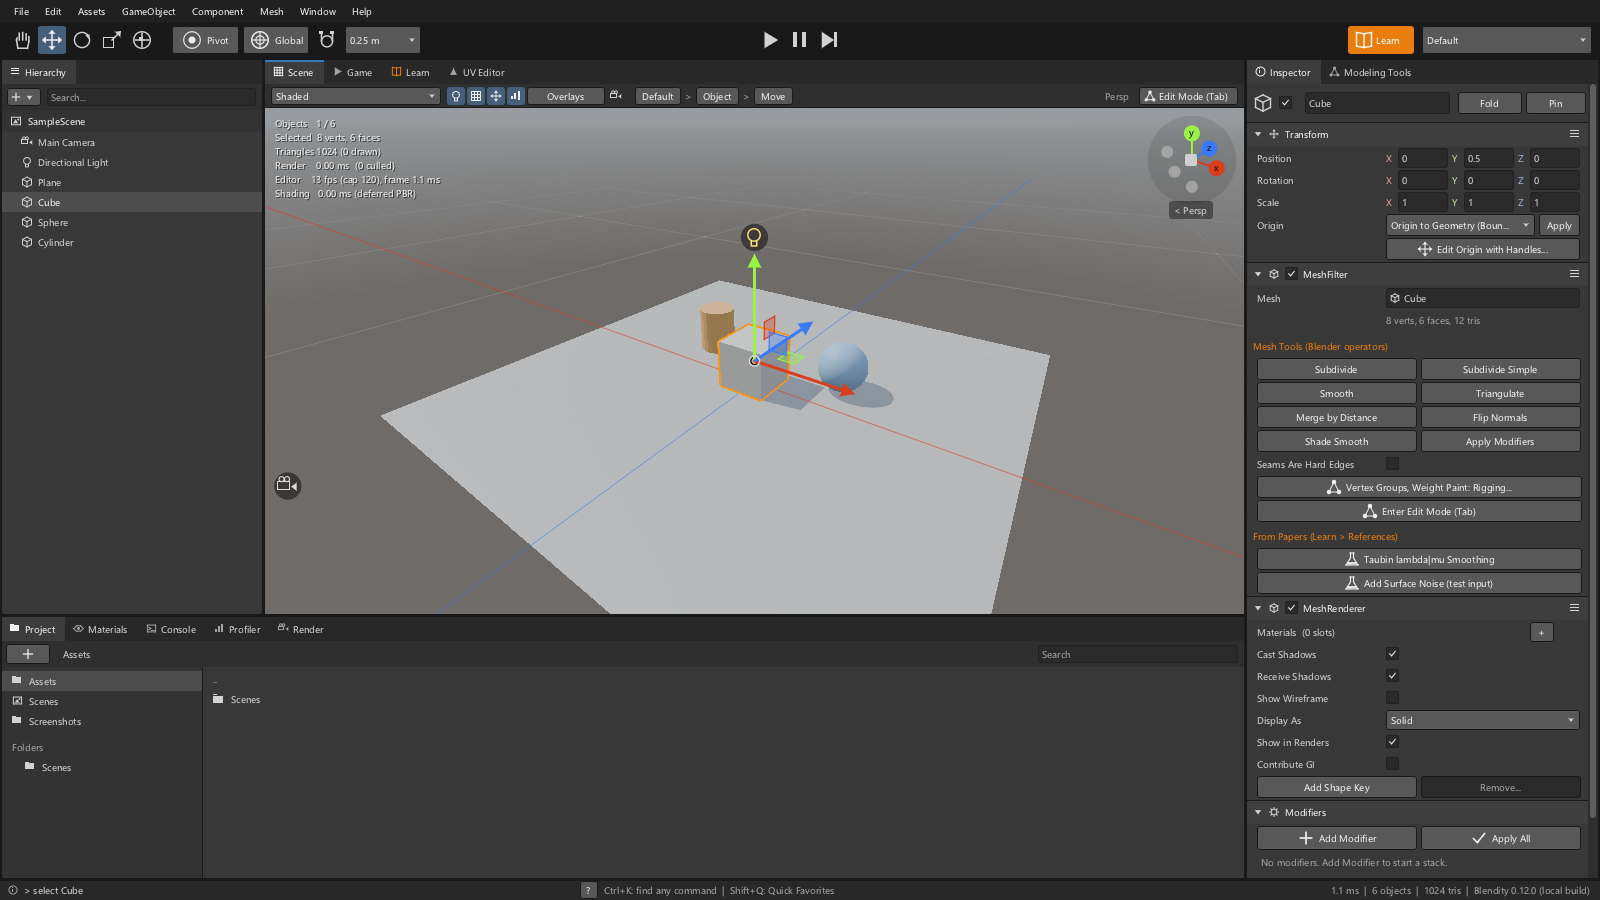
\includegraphics[width=0.86\textwidth, alt={The Default layout of the Blendity editor: Hierarchy, Scene view, Inspector and Modeling Tools, Project and Console; the toolbar's tools, pivot, space and snap increment; Play, Pause and Step; the Learn button and the Layout dropdown at the top right.}]{editor-default.png}\par
  \vspace{14mm}
  {\sffamily Emiliano Manalo, with Anthropic's Claude\par}
  {\sffamily Version 0.13.0 \quad November 2026\par}
  \vfill
  {\sffamily\footnotesize Blendity is free software (GPL). Your scenes, meshes, textures and renders are yours. \url{https://github.com/EmilianoManaloIV/blendity}\par}
\end{titlepage}

\chapter*{How to read this guide}
\addcontentsline{toc}{chapter}{How to read this guide}
Blendity is a 3D editor that works like Unity (windows, navigation, gizmos, the Inspector, Play mode) and models,
unwraps, textures, renders, rigs and animates the way Blender does. This guide takes you through the editor in the
order you will meet it: installing it, finding your way around, and then the work stage by stage. If you come from
another program, chapter~\ref{ch:comingfrom} is written for you: it puts your keys and your habits beside Blendity's and
says what is where.

Three things to know before you start. \textbf{The Learn tab} (\key{F1}) teaches every part of the editor
interactively, with Try-it buttons that drive the editor while you watch; this guide names the lesson to open at the
end of each chapter. \textbf{The command palette} (\key{Ctrl+K}) finds any command by name, with its shortcut beside it.
\textbf{Nothing is hidden for good}: a stage's layout shows that stage's tools first, and \menu{Window > Layouts > Show
All Tools} shows everything.

\textbf{Conventions.} \key{Ctrl+K} is a key or a chord; \menu{Window > Layouts} is a path through the menus;
\ui{Generate Lighting} is a button, field or window as it is labelled; \code{select Cube} is a console command, a file
or a path; a \emph{Learn} box at the end of a chapter names the lessons to open next; a ``Coming from'' box says what a
Unity or Blender user should know at that point; an ``Example'' box is a short task to follow step by step.

Every idea Blendity borrows is credited: the References chapter lists the papers, books, manuals and programs behind
the features, with the pages where each is used, and Index C ties each Learn lesson to its sources.

\tableofcontents
\listoffigures

\mainmatter
\chapter{Installing Blendity and the first start}
\label{ch:install}

Blendity is free. You don't need Blender or anything else: the installer brings everything Blendity uses. Version
0.13.0 is a \textbf{pre-release}: it works, but it is still being refined, so expect rough edges and save your work
often.

\section{Download}
Open the Releases page, \url{https://github.com/EmilianoManaloIV/blendity/releases}, or click the link for your
computer in the project's README: it fetches the one file you need, always the newest version.

\begin{center}
\begin{tabular}{ll}
\toprule
Your computer & The file \\
\midrule
Windows 10 or 11 & \code{Blendity-Setup-Windows.exe} \\
A Mac with an Apple chip (M1 or later) & \code{Blendity-macos.dmg} \\
Linux (Ubuntu 22.04 or newer, Fedora, Mint, \ldots) & \code{Blendity-linux-x86\_64.AppImage} \\
\bottomrule
\end{tabular}
\end{center}

Not sure which Mac you have? Apple menu $>$ About This Mac: ``Chip: Apple M\ldots'' means an Apple chip. Macs with an
Intel processor aren't supported yet. Every release also carries \code{SHA256SUMS.txt} (Blendity's updater checks
downloads against it), this guide and the architecture book as PDFs, and ``Source code'' archives that are for
developers.

\section{Install}
\textbf{Windows.} Double-click \code{Blendity-Setup-Windows.exe}. If a blue box says ``Windows protected your PC'', click
\ui{More info}, then \ui{Run anyway} (Blendity isn't signed with a paid certificate yet). Pick \ui{for me only} if asked
(no administrator needed), accept the licence, keep \ui{Blendity with Blender's libraries (recommended)}, tick a
desktop shortcut if you want one, \ui{Install}, \ui{Finish}. Next time, open it from the Start menu. To uninstall:
Settings $>$ Apps $>$ Installed apps $>$ Blendity $>$ Uninstall; your projects are kept.

\textbf{Mac.} Double-click the \code{.dmg}, drag \ui{Blendity} onto \ui{Applications}, open it from Applications. The
first time macOS says it can't check the app: on macOS 15 or newer click \ui{Done}, then System Settings $>$ Privacy \&
Security $>$ \ui{Open Anyway}; on macOS 14 or older right-click Blendity $>$ \ui{Open} $>$ \ui{Open}. If macOS says
Blendity ``is damaged'', run \code{xattr -dr com.apple.quarantine /Applications/Blendity.app} in Terminal once. To
uninstall, drag it to the Bin.

\textbf{Linux.} Right-click the \code{.AppImage} $>$ Properties $>$ Permissions $>$ \ui{Allow executing file as program},
then double-click it. If nothing happens, download the plain folder (\code{blendity-linux-x86\_64.tar.gz} from the
``libraries'' release), extract it and double-click \ui{Blendity} inside. To uninstall, delete the file or the folder.

\section{The first start}
\begin{itemize}
  \item The welcome asks \textbf{where you come from} (Unity, Unreal, Blender, Photoshop \& Substance) and sets the keys and
    the editor feel together; Help $>$ Welcome asks again, and chapter~\ref{ch:comingfrom} explains each choice.
  \item Your work is saved in a \textbf{project folder}: \code{BlendityProject} in your home folder unless you open
    another. A project is just a folder with \code{Assets} inside, like Unity's; copy it to another machine and open a
    scene in it. The program's folder belongs to the installer; your scenes, materials and renders never live there.
  \item Press \key{F1} for the \textbf{Learn tab}: short interactive lessons for each part of Blendity, with Try-it
    buttons that drive the editor while you watch (chapter~\ref{ch:learn}).
  \item \textbf{Updates:} once a day, when online, Blendity asks GitHub whether a newer build exists and shows what it
    brings with \ui{Install} / \ui{Not now} / \ui{Skip this one}; installs are checked against the release's SHA-256
    list. Help $>$ Version History goes back to an older version if a new one gives you trouble. Preferences $>$ Updates
    turns the check off or limits it to stable releases.
  \item \textbf{With or without Blender's libraries:} an install holds two programs, Blendity (its own code only, always
    starts) and Blendity-full (with Blender's libraries: faster ray tracing, denoising, OpenColorIO's views, Jolt
    physics, video export, Booleans, Decimate, EXR). Blendity starts first and hands over to the full one when its
    libraries load and you want them; offline, or with a library missing, it runs on its own code and says so.
    Preferences $>$ Libraries is your choice; \code{--no-libs} starts without them once; when they are missing and you
    are online, Blendity offers to download them for this build.
  \item \textbf{On a small laptop} (the HP Envy 13-inch 2-in-1 class: 4 cores, 8~GB, Iris Xe) Blendity starts on the
    \ui{Low} quality tier and says so, with \ui{High} one click away (chapter~\ref{ch:trouble}).
\end{itemize}

\section{Starting from the command line}
\begin{lstlisting}[language=console]
Blendity --layout Learning            # start with the Learn tab beside the Scene view
Blendity --scene Assets/Scenes/SampleScene.scene
Blendity --scale 1.5                  # force the UI scale (the default follows the OS DPI)
Blendity --headless-screenshot out.png --cmd "select Cube" --cmd "shading rendered" --frames 30
\end{lstlisting}
The last form runs with no window: it executes console commands and writes a picture, which is how the tests, the
figures in this guide and the comparison harnesses drive the editor.

\section{Privacy}
Blendity sends nothing about you or your work anywhere. The one network use it makes on its own is the optional daily
update check. There is no telemetry and no cloud; the only learned model in the program is the optional, local AI
Inbetweening download, which never changes a scene on its own (\code{docs/AI\_DISCLOSURE.md}).

\begin{fromnote}{Learn}
\emph{Welcome to Blendity}: how this editor and the Learn tab work, installing and sharing, updates and older versions,
with or without Blender's libraries.
\end{fromnote}

\chapter{Getting around}
\label{ch:windows}

\begin{figure}[H]
  \centering
  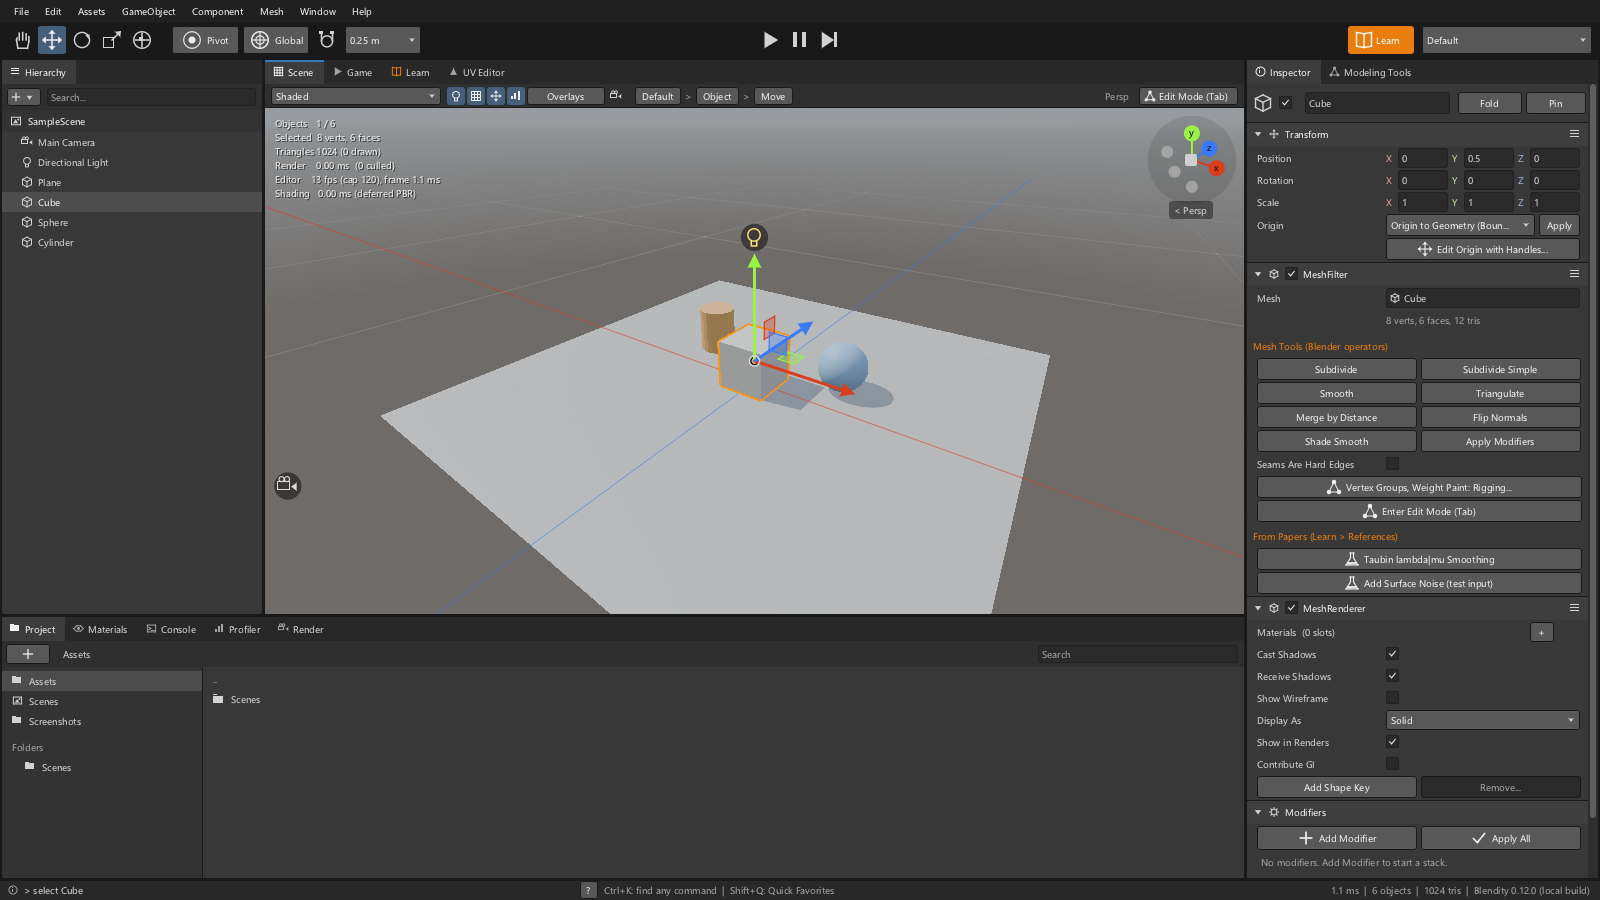
\includegraphics[width=\textwidth, alt={The Default layout of the Blendity editor: Hierarchy, Scene view, Inspector and Modeling Tools, Project and Console; the toolbar's tools, pivot, space and snap increment; Play, Pause and Step; the Learn button and the Layout dropdown at the top right.}]{editor-default.png}
  \caption{The Default layout: Hierarchy, Scene view, Inspector and Modeling Tools, Project and Console; the toolbar's
  tools, pivot, space and snap increment; Play, Pause and Step; the Learn button and the Layout dropdown at the top right.}
  \label{fig:default}
\end{figure}

\section{The windows}
\textbf{Scene} is the 3D view you edit in; \textbf{Game} shows what the active camera sees; \textbf{Hierarchy} is the
objects as a tree; \textbf{Inspector} the selected object's components; \textbf{Project} the files in \code{Assets};
\textbf{Console} the messages and a command line. Under \menu{Window} are the UV Editor, Render, Materials, Textures,
Modeling Tools, Lighting, Rigging, Animation, Sequencer, Live Link, Editing, History, Profiler, Draw, Layers, Board,
Avatar, My Tools and Learn windows. Drag a tab onto another tab bar to group it, onto a panel's edge to split it, out
past the editor's edge for a window of its own on any display; middle-click a tab to close it; right-click it for more.

\begin{fromnote}{Coming from Unity}
These are Unity's windows under Unity's names, docked the same way. \textbf{Modeling Tools} is the window Unity does
not have: every modeling, sculpting, painting and drawing tool lives there (and in the \menu{Mesh} menu), grouped by
stage.
\end{fromnote}
\begin{fromnote}{Coming from Blender}
Scene view = 3D Viewport; Hierarchy = Outliner; Inspector = Properties editor (modifiers and materials are there too);
Project = File / Asset Browser; Console = Info editor; the Layout dropdown = Workspaces. Areas split by dragging an edge
as in Blender; tabs dock as in Unity.
\end{fromnote}

\section{Layouts for each stage}
The \ui{Layout} dropdown (top right) arranges the windows for a stage of the work and shows that stage's tools and tabs
first, so the editor never feels like every tool at once. Nothing is ever gone: hidden tools still answer their keys and
the palette, \menu{Window > Layouts > Show All Tools} shows everything, and \ui{Save Layout\ldots} keeps your own.

\begin{center}
\begin{tabularx}{\textwidth}{lXX}
\toprule
Layout & Windows & Tools shown \\
\midrule
Default & everything & everything \\
Reference \& Planning & Scene, Game, Project, Board & create, reference images, cameras \\
Blocking Out & Scene, Modeling Tools & primitives, drawing, snapping \\
Modeling \& Topology & Scene, Modeling Tools & Edit Mode, checks, curves and lattices \\
UV Unwrapping & Scene beside the UV Editor & Edit Mode, UVs \\
Texturing \& Materials & Scene, Game, Materials, Textures & materials, textures, baking \\
Texturing, Stylized & Scene, Textures / Modeling Tools & surfaces, paint; strokes, scatter, sky \\
Lighting \& Rendering & Scene, Game, Lighting, Render & lights, cameras, bakes \\
Editing & Editing, Render & developing a render \\
Rigging; Skinning \& Weight Painting & Scene, Game, Rigging & bones, skins, IK, deformers; weights \\
Animation & Scene, Game, Animation along the bottom & animation, rigging, puppet posing \\
Drawing; Drawing with References & Draw, Layers, (Board) & the pen's pad, its layers, the board \\
Learning & Learn beside the Scene view & everything \\
\bottomrule
\end{tabularx}
\end{center}

In one area, Materials, Textures and Lighting fold into one \ui{Shading} tab with a row of the three under it (Rigging
\& Animation and Tools fold the same way; \ui{Fold Groups} in the tab menu turns it off). A tab strip whose labels don't
fit shows the inactive tabs as icons, then lists the rest under $\gg$; the stage's hidden tabs sit under $+N$. The
Scene view's bar reads \emph{Layout $>$ Mode $>$ Tool}, each part a dropdown.

\begin{figure}[H]
  \centering
  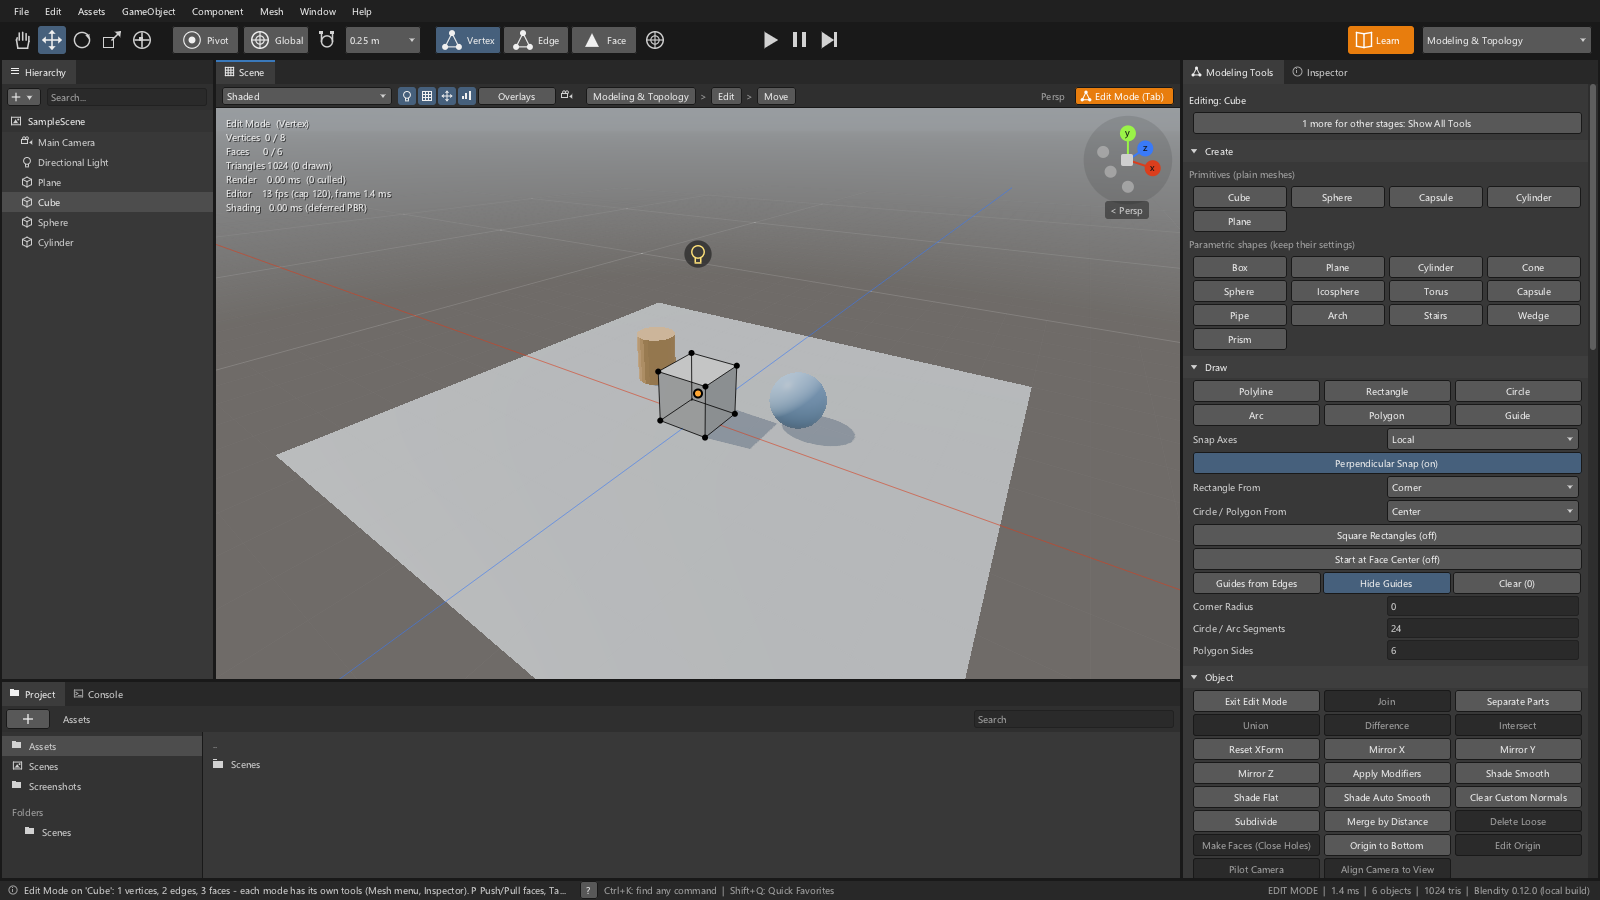
\includegraphics[width=\textwidth, alt={The Modeling and Topology layout with a cube in Edit Mode: the Scene view with the cube's cage and the Edit Mode bar, the Modeling Tools window listing the Select, Create and Extrude, Cut and Divide and Merge and Clean Up sections, the Draw tools and the checks.}]{layout-modeling.png}
  \caption{The Modeling \& Topology layout in Edit Mode: the Modeling Tools window shows the Edit Mode sections (Select,
  Create \& Extrude, Cut \& Divide, Merge \& Clean Up), the Draw tools and the checks.}
\end{figure}

\section{Navigating}
With Unity's mouse (the default feel): \key{Alt}+left drag orbits, middle drag pans, the wheel zooms, hold the right
button and use \key{W A S D} (\key{Q} / \key{E} down and up, \key{Shift} faster) to fly, \key{F} frames the selection. Click
the cones of the gizmo in the corner for front, top and side views, its centre for perspective or orthographic.
\menu{Edit > Editor Feel} switches the mouse navigation and the keys together to Unreal's, Blender's or Maya's
(chapter~\ref{ch:comingfrom}).

\section{Selecting and moving}
Click to select, \key{Ctrl}+click to add, drag a box. \key{Q W E R Y} pick the View, Move, Rotate, Scale and Transform
tools; Blender's \key{G} / \key{R} / \key{S} also work, with \key{X} / \key{Y} / \key{Z} to lock an axis and a typed number
(the Blender keys for R and S are a preference, since R is Unity's Scale tool). Hold \key{Ctrl} to snap (the increment is
the dropdown beside the magnet); \key{Ctrl+Shift} while moving drops the object onto the surface under the mouse;
\key{V} snaps a vertex onto another. While dragging a gizmo arrow, type a number to move exactly that far.

\section{Objects, components and the Inspector}
As in Unity, everything in a scene is a GameObject with a Transform; what it does comes from its components
(MeshFilter, MeshRenderer, Light, Camera, Rigidbody, Animation, modifiers, Camera Filters, \ldots). Create objects from
the Hierarchy's right-click menu or the \menu{GameObject} menu; drag a Hierarchy row onto another to parent it (in
thirds: above, into, below). The Inspector shows each component's first seven fields and keeps the rest under
\ui{Show more}; \ui{All Fields} shows everything. Number fields take expressions: \code{2*pi}, \code{+=1}, \code{*=2}
(relative to each object's own value), \code{L(0,10)} (spread evenly across the selection), \code{R(0,1)} (random per
object); with several objects selected a change applies to all of them. A field that names another object takes a typed
name or a row dragged from the Hierarchy; an asset field takes a file dragged from the Project window. Right-click a
field's name for \ui{Reset to Default} or \ui{Insert Keyframe}.

\section{Origins, Play, undo}
\menu{GameObject > Set Origin} moves the pivot to the bounds centre, the median, the centre of mass, the bottom centre,
a point, the edit selection or the view pivot without moving anything on screen; \ui{Edit Origin (Handles)} moves only
the origin with the gizmo and snaps it to vertices, edges and faces. \key{Ctrl+P} plays the scene; changes made while
playing are thrown away on Stop, as in Unity. \key{Ctrl+Z} / \key{Ctrl+Y} undo and redo the scene, materials, textures
and clips as one step per operation; \menu{Window > History} lists every step and a click goes back to it.

\section{Finding anything: the palette, favorites, the Wheel}
\key{Ctrl+K} (or \key{F3}, Blender's key) opens the \textbf{command palette}: type a few words and every action, window,
layout, creatable object and console command that matches is listed with its shortcut; \key{Enter} runs it, even a tool
the current layout hides. Right-click a row (or any menu row) for its small menu: \textbf{Quick Favorites} (\key{Shift+Q},
one list per layout), \textbf{the Wheel} (\key{Space}: one radial menu for where the mouse is, with a set per mode you
fill from any menu), \textbf{My Tools} (a window of your own panels, each a grid of commands), \textbf{Assign
Shortcut\ldots} (the next key you press binds it). Preferences $>$ UI file saves the whole arrangement (layout, windows,
feel, keymap and your shortcuts, panels, the Wheel's sets, favorites, theme, scale) as one \code{.blendity-ui} file.

\section{The status bar, toasts and the job tray}
The status bar says what the mouse and keys do where the mouse is and offers Undo for the last action; the \ui{?}
beside the hint opens the Learn lesson for what you are doing. A warning is a toast over the Scene view for three
seconds, with a \ui{Fix} button when a command puts it right (stop Play, cancel the job, unwrap first); a button that
cannot work now is dim and its tooltip says why. A long job (a bake, a remesh, a render, an export) shows in the status
bar's right slot with its progress, the time run, an estimate left and \ui{Cancel}; a toast says when it ends. The
results of checks (UV Report, Scene Statistics, Motion Check) open in a \ui{Report} dialog.

\section{Windows on other screens and Tablet Mode}
Drag any tab out past the editor's edge for a window of its own where you let go; right-click a tab for \ui{Move to New
Window}, \ui{Move to Display N} or \ui{Move to Main Window}. A Render or Game tab in its own window can be \ui{Render
Only} and \ui{Full Screen}: a second monitor showing the render large. The Scene view, the Game view and the Inspector
can be \ui{duplicated} into a new window; a second Inspector has a \ui{Pin} that keeps one object while the selection
moves on. \textbf{Tablet Mode} (the tab menu, or Preferences $>$ Pen and touch: Auto turns it on when a 2-in-1's
keyboard folds away) makes the targets half as big again, and then fingers navigate (one orbits, two pinch, pan and
twist) while the pen selects, moves, draws and paints (chapter~\ref{ch:pen}).

\section{Themes}
Preferences $>$ Theme: Dark, Light, Emiliano Light, Emiliano Dark (the palette of the author's site: paper, charcoal
and an amber accent) and High Contrast (white on near-black with every text at WCAG's 4.5:1 or more
\cite{W3C2018Web} and a yellow focus ring; the tests measure every theme's ratios).

\begin{fromnote}{Learn}
\emph{The Editor Layout}, \emph{Navigating the Scene View}, \emph{GameObjects, Components and Objects},
\emph{Hierarchy, Parenting and the Scene Graph}, \emph{Move, Rotate, Scale}, \emph{Customizing the Editor},
\emph{Undo, Selection and Memory}.
\end{fromnote}

\chapter{Coming from another program}
\label{ch:comingfrom}

Blendity has two kinds of users by design: Unity users who expect Unity's navigation, its \key{W} / \key{E} / \key{R}
tools and an Inspector, and Blender users who expect to model with the keyboard. The rule that resolves the clashes
(\code{docs/USABILITY.md}) is: \textbf{move the view and pick tools as Unity does; change geometry as Blender does
(a verb key, the mouse or a typed number, click to confirm, F9 to adjust); settings in the Inspector}. Nothing a Unity
user already knows changes by default, and everything a Blender user reaches for while modeling works. The first run
asks where you come from and sets the keys and the feel; \menu{Edit > Preferences > Keymap} starts from any of seven
presets and rebinds anything; \code{keymap table} in the console prints every action's chords under every preset.

\section{The editor feel}
\menu{Edit > Editor Feel} switches the keys \emph{and} the Scene view's mouse navigation to another program's:

\begin{center}
\small
\begin{tabularx}{\textwidth}{l>{\raggedright\arraybackslash}p{16mm}>{\raggedright\arraybackslash}p{26mm}>{\raggedright\arraybackslash}p{24mm}>{\raggedright\arraybackslash}p{24mm}X}
\toprule
Feel & Orbit & Pan & Zoom / dolly & Look + fly & Its own keys \\
\midrule
Unity & Alt+LMB & MMB, Alt+Ctrl+LMB & Wheel, Alt+RMB & hold RMB + WASD & the Unity table below \\
Unreal & Alt+LMB & MMB, LMB+RMB & Wheel, Alt+RMB & hold RMB + WASD & Alt+P play, End drop to floor, Alt+G/H/J/K views \\
Blender & MMB & Shift+MMB & Wheel, Ctrl+MMB & -- & G/R/S, A, X, Shift+D \\
Maya & Alt+LMB & Alt+MMB & Wheel, Alt+RMB & -- & Q/W/E/R, F8, F9--F11 \\
\bottomrule
\end{tabularx}
\end{center}

Window names, layouts and the Y-up axis stay Unity's whatever the feel.

\section{From Unity}
\begin{fromnote}{What carries over}
Everything on the surface: the windows, Alt-orbit, \key{Q W E R Y}, \key{F} to frame, \key{Ctrl+D} duplicate, \key{Ctrl+P}
play, \key{Ctrl+Shift+N} empty, \key{Ctrl+1}\ldots\key{9} windows, the Inspector with multi-object editing, drag-and-drop of
assets, the Project window, Play mode that reverts, the Animation window (dopesheet, Curves, Record, Add Property,
\key{K} keys every track, comma and full stop step keys), Humanoid retargeting as Mecanim reads a T and an A pose,
\code{.anim} clips, \code{.unitypackage}, prefabs, scenes and \code{.mat} files read and written, LOD Groups, colliders,
Light modes (Realtime / Mixed / Baked), Contribute GI, lightmaps and probe volumes, post-processing as Camera Filters.
\end{fromnote}
What is new is \textbf{Edit Mode} (\key{Tab}) with Blender's operators (chapter~\ref{ch:model}), the \textbf{Modeling
Tools} window, \textbf{F9} to adjust the last operation, materials evaluating Blender's Principled BSDF with a layer
stack of textures instead of a shader graph, two render engines in F12, and the \textbf{Learn} tab. What is not there:
C\# scripts (Play has a few built-in behaviours and the Sequencer's triggers) and the Animator state machine (the
Sequencer's tracks and triggers do the job). A Unity scene opened here looks as its Game view does, and Live Link sends
your work back into a Unity project as you edit (chapter~\ref{ch:files}).

\section{From Blender}
\begin{fromnote}{What carries over}
The data and the tools: the mesh with n-gons, per-corner UVs and seams; \key{Tab}, \key{1} / \key{2} / \key{3}, \key{G} and
the axis keys with typed values, \key{E} extrude, \key{I} inset, \key{Ctrl+B} bevel, \key{Ctrl+R} loop cut, \key{K} knife,
\key{Alt}+click loops and \key{Ctrl+Alt}+click rings, \key{F9}, \key{O} proportional editing, \key{Shift+N} normals, the
modifier stack with the same header toggles, the Principled BSDF, LSCM and Smart UV, the Hosek--Wilkie sky, Filmic and
AgX (with OpenColorIO), Cycles-like path tracing, the Graph Editor's tangent modes, bones and armatures, automatic
weights, the NLA's idea as sequences, every export format with Blender's options.
\end{fromnote}
Pick the \textbf{Blender} preset and feel: middle-mouse orbit, \key{R} rotates and \key{S} scales, \key{A} selects all,
\key{X} deletes, \key{Shift+D} duplicates, \key{F} fills, \key{M} merges, \key{J} connects, \key{L} selects linked,
\key{.} frames, \key{Shift+I} keys. Under the Unity preset \key{R} is the Scale tool (Edit $>$ Blender Transform Keys
moves Scale to \key{T}), \key{E} is the Rotate tool and \key{Ctrl+E} extrudes, \key{Alt+F} fills, \key{Alt+M} merges.
What is different in kind: windows dock as Unity's and layouts replace workspaces; the Inspector replaces the N panel
and the redo panel (tool numbers live in F9 or the drag helper, not the Inspector); the axes are Unity's (Y up,
left-handed: OBJ and FBX mirror X on the way out as Unity's importer does); there is no node editor (chapter~\ref{ch:surface}
maps Blender's texture and converter nodes to layers), no Python (the console), no \code{.blend} except through your
installed Blender (\code{import file.blend}), and Live Link sends the scene into Blender live.

\section{From Maya}
Pick the \textbf{Maya} preset and feel: Alt+LMB orbit, Alt+MMB pan, \key{Q W E R} tools, \key{F8} toggles components
(Edit Mode), \key{F9} / \key{F10} / \key{F11} vertex / edge / face (so Adjust Last moves to \key{Ctrl+F9} and the Render
window leaves F11), \key{S} sets a key, \key{B} soft select (proportional editing), \key{Ctrl+Shift+X} Multi-Cut (the
knife), \key{Ctrl+M} collapse, \key{Z} / \key{Shift+Z} undo and redo. Maya's Outliner is the Hierarchy, the Attribute
Editor the Inspector, the Hypershade the Materials and Textures windows, the Graph Editor the Animation window's Curves
view.

\section{From 3ds Max}
Pick the \textbf{3ds Max} preset: \key{Q W E R}, \key{Z} frames, \key{Tab} enters the editable poly's sub-objects (Edit
Mode), \key{1} / \key{2} / \key{4} vertex / edge / polygon, \key{Ctrl+V} clones, \key{Shift+E} extrude, \key{Shift+I}
inset, \key{Ctrl+Shift+C} chamfer (bevel), \key{Alt+C} cut (knife), \key{Ctrl+Shift+E} connect, \key{Ctrl+Alt+C}
collapse, \key{Ctrl+D} deselects. The modifier stack is the Inspector's modifier list, bottom to top as Blender's.

\section{From SketchUp}
Pick the \textbf{SketchUp} preset: \key{Space} selects, \key{M} moves, \key{Q} rotates, \key{S} scales, \key{L} line,
\key{R} rectangle, \key{C} circle, \key{A} arc, \key{Shift+P} polygon, \key{P} Push/Pull, \key{F} offset (inset),
\key{E} erases, \key{Shift+Z} zoom extents, \key{Shift+Space} the Wheel. The \textbf{Draw} tools draw onto faces or the
ground with SketchUp's inference (the axes, parallel and perpendicular edges, midpoints, face centres); a closed shape
on a face is cut into it, ready to \textbf{Push/Pull} with SketchUp's semantics (\adr{0004}, \cite{SketchUpHelp2026}):
pulled, it extrudes; pushed through, it makes a hole; pushed flush with another face, it merges; \key{Ctrl} keeps the
original face. Follow Me is \ui{Follow}, the Tape Measure's guides are \ui{Guide} and the \key{X} / \key{Y} / \key{Z}
construction lines; groups and components are objects and child objects; \textbf{N-gon Mode} treats each flat region
as one face as SketchUp does.

\section{From Unreal}
Pick the \textbf{Unreal} preset and feel: Unity's keys with Unreal's on top (\key{Alt+P} plays, \key{Ctrl+W} duplicates
too, \key{End} drops the selection to the floor, \key{Alt+G/H/J/K} the perspective, front, top and side views, LMB+RMB
pans). The Outliner is the Hierarchy, the Details panel the Inspector, the Content Browser the Project window, the
Sequencer is here under the same name (clips, cards, camera cuts, sound), Post Process Volumes are Camera Filters. Live
Link sends the scene into a level through the Unreal bridge (lights, cameras, LODs and UCX collision as Unreal names
them), and \ui{Send to Blendity} brings a level back.

\section{From Photoshop, Substance Painter and SketchBook}
Pick the \textbf{Adobe} preset: Unity's keys with Photoshop's brush keys on top \cite{PhotoshopHelp2026}: \key{B}
enters Paint Mode (and leaves Sculpt), \key{E} toggles the eraser (or Carve in Sculpt), \key{V} is the Move tool, \key{H}
the Hand tool, \key{[} / \key{]} the brush size (in every preset), \key{Shift+[} / \key{]} its opacity, \key{Ctrl+T}
Free Transform, \key{Space} held pans, \key{Ctrl+0} fits. The \textbf{Draw tab} works like SketchBook Pro's canvas
\cite{SketchBookDocs2026} with Photoshop's 27 blend modes, clipping and layer masks, rectangle and lasso selections
and Illustrator's shapes and Pen (chapter~\ref{ch:pen}). The \textbf{Textures} window's surfaces are Substance
Painter's pipeline \cite{SubstancePainterDocs2026}: bake mesh maps, fill layers with mask stacks reading them, smart
masks and smart materials, a material brush that paints colour, roughness, metallic, height and emission at once, and
a texture set exported in the glTF, Unity, URP, HDRP, Unreal, Poiyomi or lilToon packing (chapter~\ref{ch:surface}).
The \textbf{Editing} tab develops a render as Lightroom does. The \textbf{Board} is a PureRef-style reference board
\cite{PureRef2026}.

\section{The shortcut table}
The table below is the Unity preset beside Blender's own keys; \code{keymap table} prints every preset.

\begin{center}
\small
\begin{tabularx}{\textwidth}{Xll}
\toprule
 & Blendity (Unity preset) & Blender \\
\midrule
Orbit / Pan / Zoom & Alt+LMB / MMB / Wheel or Alt+RMB & MMB / Shift+MMB / Wheel \\
Fly & hold RMB + WASD, Q/E, Shift & Shift+` \\
Frame selection & F & Numpad . \\
Views, Persp / Iso & the scene gizmo's axes / centre & Numpad 1 / 3 / 7, Numpad 5 \\
Create objects & right-click in the Hierarchy & Shift+A \\
View / Move / Rotate / Scale / Transform & Q / W / E / R / Y & -- / G / R / S / Transform tool \\
Duplicate / Delete / Rename & Ctrl+D / Del / F2 & Shift+D / X / F2 \\
Play / Pause / Step & Ctrl+P / Ctrl+Shift+P / Ctrl+Alt+P & -- \\
Edit Mode / vertex / edge / face & Tab / 1 / 2 / 3 & Tab / 1 / 2 / 3 \\
Grab / rotate / scale (modal) & G, X / Y / Z, a typed value & G / R / S \\
Extrude / Inset / Bevel & Ctrl+E / I or Ctrl+I / Ctrl+B & E / I / Ctrl+B \\
Select edge loop / ring & Alt+click / Ctrl+Alt+click & Alt+click / Ctrl+Alt+click \\
Loop cut / Knife / Connect & Ctrl+R / K / J & Ctrl+R / K / J \\
Push/Pull (face mode) / Push Through & P / Alt+P & -- \\
Bridge & Ctrl+Shift+B & Bridge Edge Loops \\
Fill / Merge at center / Recalculate normals & Alt+F / Alt+M / Shift+N & F / M / Shift+N \\
Dissolve / Triangulate / Tris to quads & Ctrl+X / Ctrl+T / Alt+J & Ctrl+X / Ctrl+T / Alt+J \\
Proportional editing & O & O \\
Adjust Last Operation & F9 & F9 \\
Set a key / Record / prev, next key & Shift+K / Ctrl+Shift+K / , . & Shift+I / -- / Down, Up \\
UV Editor / Unwrap & Ctrl+9 / U & UV Editing workspace / U \\
Render / Render window / Render Animation & F12 / F11 / Ctrl+F12 & F12 / F11 / Ctrl+F12 \\
Palette / Favorites / the Wheel & Ctrl+K or F3 / Shift+Q / Space & F3 / Q / -- \\
Learn & F1 & -- \\
\bottomrule
\end{tabularx}
\end{center}

\begin{fromnote}{Learn}
\emph{Navigating the Scene View} (the shortcut sheet), \emph{Coordinate Systems and Handedness}, \emph{Edit Mode:
Modeling Like Blender}, \emph{Customizing the Editor}.
\end{fromnote}

\chapter{Reference, planning and blocking out}
\label{ch:plan}

\section{Reference images and the board}
\menu{GameObject > Reference Image\ldots} puts a picture into the scene as an unlit plane facing the front, sized to
the picture, kept out of renders and shadows (\code{refimage <path> front|side|top} picks the view). A picture from
outside the project is copied into \code{Assets/Textures/References}, so the scene keeps it on another machine. The
\textbf{Board} (\menu{Window > Board}, or the Drawing with References layout) is a reference board in PureRef's way
\cite{PureRef2026}: drop images from the system, paste a screenshot with \key{Ctrl+V} or drag them from the Project
window onto an endless canvas; move, scale and turn them by their handles; it saves itself to \code{Assets/Boards} and
opens again next time. \menu{Boards > Export\ldots} writes it as PNG, JPEG or PDF.

\begin{example}{model from a front and a side drawing}
\begin{enumerate}
  \item Layout $>$ Reference \& Planning.
  \item \menu{GameObject > Reference Image\ldots}, pick the front drawing; for the side drawing type \code{refimage
    <path> side} in the Console.
  \item Scale and move the planes so the drawings line up (the Inspector's Scale field takes \code{*=2}).
  \item Switch to Blocking Out and start with primitives over them.
\end{enumerate}
\end{example}

\section{Cameras and shots}
Add a Camera (\menu{GameObject > Camera}: it is placed at the view, looking its way) and pick it in the Game view's
camera menu; selecting a camera shows a \textbf{Camera Preview} in the corner of the Scene view. \textbf{Pilot Camera}
flies the Scene view as that camera; composition guides (thirds, golden ratio, safe areas) draw over its frame.
Physical camera settings (focal length, sensor presets, f-stop, focus distance, blades, shift) are in the Camera's
Inspector; the focus eyedropper focuses on the surface you click, and Pick Focus Point keeps a world point in focus.
The scene's \textbf{Active Camera} is what F12 and the Game view use.

\section{Blocking out}
\menu{GameObject > 3D Object} is in every layout: cube, sphere, icosphere, cylinder, cone, torus, plane, quad, capsule
and the Utah teapot \cite{Newell1975Utilization}. \menu{GameObject > Shapes (Parametric)}: box, plane, cylinder, cone,
sphere, icosphere, torus, capsule, pipe, arch, stairs, wedge and prism keep their settings in the Inspector and rebuild
as you change them, like ProBuilder's shapes \cite{ProBuilderDocs2026}. Right after adding a primitive, the
\textbf{Adjust Last} panel at the bottom left of the Scene view (\key{F9}) changes its size, segments or rings as one
undo step.

\textbf{Drawing, SketchUp-style.} The Draw tools (Polyline, Rectangle, Circle, Arc, Polygon) draw onto faces or the
ground with snapping to corners, midpoints, edges, face centres and the drawing plane's axes; \key{X} / \key{Y} / \key{Z}
lay construction lines; \key{Ctrl}+click lays a guide along an edge; rectangles come from a corner, the centre or three
points; circles from the centre, a diameter or three points. A closed shape on a face is cut into it, ready to
\textbf{Push/Pull} (\key{P}): move the mouse or type a distance, click to confirm. Pushed through, it makes a hole,
imprinted on whatever face it exits through; pulled onto another face, it joins it; \key{Ctrl} keeps the original face.
\cite{SketchUpHelp2026, UModelerDocs2026, PlasticityDocs2026}

\textbf{Booleans} (with Blender's libraries: the Manifold solver). Select the cutters, then \key{Ctrl}+click the object
to cut last; \menu{Mesh > Boolean} (Union, Difference, Intersect) applies at once or adds a live modifier whose cutter
stays editable as a wire outline. \textbf{Join} (\key{Ctrl+J}) combines meshes; \textbf{Separate} splits off the
selection or each loose part. From UModeler and Plasticity: \textbf{Follow} (sweep a face along a path), \textbf{Spin /
Lathe}, \textbf{Slice}, \textbf{Shell}, \textbf{Thicken}, \textbf{Draft}, a \textbf{Radial Array}; \textbf{Smart Fill}
closes holes and wire loops. Hold \key{Ctrl} for grid snapping; \key{Ctrl+Shift} while moving drops an object onto the
surface under the mouse.

\begin{example}{a doorway in a wall}
\begin{enumerate}
  \item \menu{GameObject > Shapes (Parametric) > Box}; in the Inspector make it 4 $\times$ 3 $\times$ 0.2.
  \item Select the box, \ui{Rectangle} (Modeling Tools $>$ Draw), and draw a rectangle about 1 $\times$ 2.1 on its front
    face from the bottom edge (hold \key{Ctrl} to snap; the length shows as you draw).
  \item Press \key{P} over the rectangle and push it through the wall: the doorway is cut.
\end{enumerate}
\end{example}

\section{Drawing in perspective, building from the construction}
For a drawing pad or a pen: \menu{Draw > Sketch (pen)} draws over the Scene view with SketchBook's aids under
\menu{Draw > Guides} \cite{SketchBookDocs2026}: a ruler, an ellipse, French curves, symmetry, and 1-, 2- and 3-point
perspective with draggable vanishing points. When the pen lifts the stroke is corrected to what it meant
\cite{Igarashi1997Interactive}: split at its corners, each piece a line, an arc, an ellipse or a curve, pulled
vertical, horizontal or onto a vanishing line, its ends joined to other strokes'. The 3-point guide \emph{is} the
camera: orbit and its points move; drag a point and the camera turns to put it there. A \textbf{canvas} can be a plane
in the scene (the ground, a face, a wall through a point) and a stroke on it sits in the scene from every view; a line
along the plane's axis becomes a construction line. \menu{Draw > Build from Sketch} makes solids from the strokes that
fix them, 3-Sweep's way \cite{Chen2013Sweep}: a box from three lines at a corner, a cylinder or cone from two
circles, a sweep from two circles and a path, a face from a closed outline and its Push/Pull from a line along its
normal, with their numbers in F9. \menu{Draw > Sketch over the Model} keeps a drawing true from its view and traces a
stroke into a cut or a curve; \code{sketchlift} lifts a whole scaffold drawn under the 3-point guide into a wire object
\cite{Gryaditskaya2020Lifting}. Nothing is guessed: the model is built by the artist's own steps.

\begin{example}{a box from a drawing}
\begin{enumerate}
  \item \menu{Draw > Sketch (pen)}; \code{sketchcanvas ground}. Draw two lines from one point along the red and the blue
    axis (they snap along the axes and become construction lines).
  \item \code{sketchcanvas plane z 0 0 0} (a wall through the origin) and draw the upright from the same corner.
  \item \menu{Draw > Build from Sketch > Box}: the box stands on the three lines; \key{F9} corrects its lengths.
\end{enumerate}
\end{example}

\begin{fromnote}{Learn}
\emph{Cameras and Projection}, \emph{Points, Lines, N-gons and Booleans}, \emph{Move, Rotate, Scale}, \emph{Drawing in
Perspective}, \emph{Papers}.
\end{fromnote}

\chapter{Modeling, sculpting and UVs}
\label{ch:model}

\section{Edit Mode}
\key{Tab} enters Edit Mode; \key{1} / \key{2} / \key{3} pick vertex, edge and face selection. The tools follow the
selection mode, as in ProBuilder and Blender:

\begin{center}
\begin{tabularx}{\textwidth}{llX}
\toprule
Do & Unity keymap & What it does \\
\midrule
Extrude & Ctrl+E & pull new geometry out of the selection; a lone vertex grows an edge, an edge a face \\
Inset & I / Ctrl+I & a smaller face inside each face (or the selection as one region) \\
Bevel & Ctrl+B (wheel: segments) & round or chamfer edges, with a profile from concave to convex \\
Loop cut & Ctrl+R over an edge & cut a ring of new edges round the mesh \\
Knife / Line & K & split a face between two points with endpoint, midpoint and on-edge snapping \\
Bridge & Ctrl+Shift+B & join two faces or two holes with a tube \\
Merge at center / Fill & Alt+M / Alt+F & collapse vertices, close holes (Smart Fill on open loops) \\
Dissolve / Connect & Ctrl+X / J & remove edges keeping the surface; cut between two vertices \\
Select loop / ring & Alt+click / Ctrl+Alt+click & edge loops and rings; face loops in face mode \\
Push/Pull / Push Through & P / Alt+P & SketchUp's face operator; a hole along the normal \\
\bottomrule
\end{tabularx}
\end{center}

Every modal operator behaves the same way: start with the key; move the mouse or type a number (\key{X} / \key{Y} /
\key{Z} lock an axis, twice for the local axis; \key{Shift}+axis locks a plane; \key{Ctrl} snaps; \key{Shift} is fine
control; during a bevel the wheel sets the segments, or \key{]} / \key{[} without one); a click or \key{Enter} confirms;
\key{Esc} or a right-click cancels leaving no undo step; then \textbf{Adjust Last Operation} (\key{F9}) changes the
values afterwards as the same step and remembers them as the tool's defaults. A hint bar at the bottom of the Scene
view lists the keys while any of them runs. \textbf{Proportional editing} (\key{O}) moves nearby vertices with a falloff.
\textbf{N-gon Mode} treats each flat region as one face, as SketchUp does. Shift+drag a gizmo handle extrudes first.

\textbf{Modifiers} stack non-destructively, top to bottom, as in Blender: Array (with Fit Length / Fit Curve), Bevel,
Boolean, Decimate, Mirror, Screw, Solidify, Subdivision Surface \cite{Catmull1978Recursively}, Triangulate,
Wireframe, Weld; and the deformers Cast, Curve, Displace, Lattice, Mesh Deform, Simple Deform and Smooth. Each has
Edit Mode / Viewport / Render toggles and a header as Blender's; drag a modifier's name to move it; Apply works on one
modifier ignoring those above it. \textbf{Curves and lattices}: \menu{GameObject > Curve} makes Bezier, circle and path
curves; a Lattice is a box of points that squashes the mesh inside it; their points take the same keys as vertices.

\textbf{Checks.} Select Overlapping and the Z-fighting check find faces on top of each other; Delete Loose removes stray
vertices; Recalculate Normals (\key{Shift+N}) faces everything outwards; Auto Smooth shades by angle; Select Similar
and Select by Material; \menu{Mesh > From Papers} has the tools built from research papers (Taubin smoothing
\cite{Taubin1995Signal} and others).

\begin{example}{a rounded table top}
\begin{enumerate}
  \item Create a Cube, scale it to 1.6 $\times$ 0.05 $\times$ 0.9.
  \item \key{Tab} into Edit Mode, \key{2} for edges, \key{Ctrl+Alt}+click one of the four vertical edges (an edge ring).
  \item \key{Ctrl+B} and drag; scroll for segments. \key{F9} to set the width exactly.
\end{enumerate}
\end{example}

\section{Sculpting}
\menu{Modeling Tools > Sculpt} (\code{sculpt on}) is ZBrush's workflow on the mesh under the pen \cite{ZBrushDocs2026}:
brushes (Clay Buildup, Draw, Inflate, Smooth, Grab, Snake Hook, Crease, Flatten, Scrape, Pinch) with Mirror symmetry
and Radial, a lazy mouse, image alphas and stroke types (Dots, Drag Dot, Drag Rect, Freehand, Spray); masks (\key{Ctrl}
paints, \key{Ctrl+I} inverts) that keep a brush off a region; polygroups in the eight colour-universal colours
\cite{Okabe2008Color} and hiding (\key{H} / \key{Alt+H}) to work on a part alone; a stroke one light undo step; the
pen's pressure, tilt and eraser end (the \key{[} / \key{]} keys step the size). Four ways to add resolution:
\textbf{Dynamic Subdivision} (a Catmull--Clark preview the brush edits through; the base mesh stays light),
\textbf{DynaMesh} (the shell retopologized evenly from its winding number \cite{Jacobson2013Robust,
Gibson1998Constrained}; two shapes merged into one skin), \textbf{Quad Remesh} (QuadriFlow \cite{Huang2018Quadriflow}
on a worker: a clean quad mesh at a target count, with Blender's Eigen) and \textbf{Dyntopo} (Sculptris Pro
\cite{SculptrisDocs2026}: the mesh tessellated under the brush as it moves). The pipeline order that keeps a model
clean: \emph{sculpt $>$ remesh $>$ unwrap $>$ bake mesh maps $>$ paint}; a remesh after painting would throw the paint's
UVs away.

\section{UV unwrapping}
Layout $>$ UV Unwrapping puts the \textbf{UV Editor} (\key{Ctrl+9}) beside the Scene view.
\begin{enumerate}
  \item In Edit Mode select the edges where the mesh should be cut open and \ui{Mark Seam} (or UV $>$ Seams from Sharp
    Edges).
  \item Select everything and press \key{U} to Unwrap (LSCM, as Blender's \cite{Levy2002Least}). \ui{Smart UV} projects
    by angle; \ui{Part Unwrap} finds charts by parts with ABF++ \cite{Sheffer2005Abf, Wang2025Partuv}; cube, cylinder,
    sphere and view projections are there too.
  \item In the UV Editor move, rotate and scale islands with the gizmo (\key{W} / \key{E} / \key{R}); \ui{Pack} fits them in
    the square; \ui{Avg Scale} evens them; the \ui{Stretch} overlay shows where a texture would distort; \ui{Sync} sets
    Edit Mode's faces from the UV selection. After Unwrap, Smart UV or Pack, \key{F9} changes the margin.
\end{enumerate}

\begin{figure}[H]
  \centering
  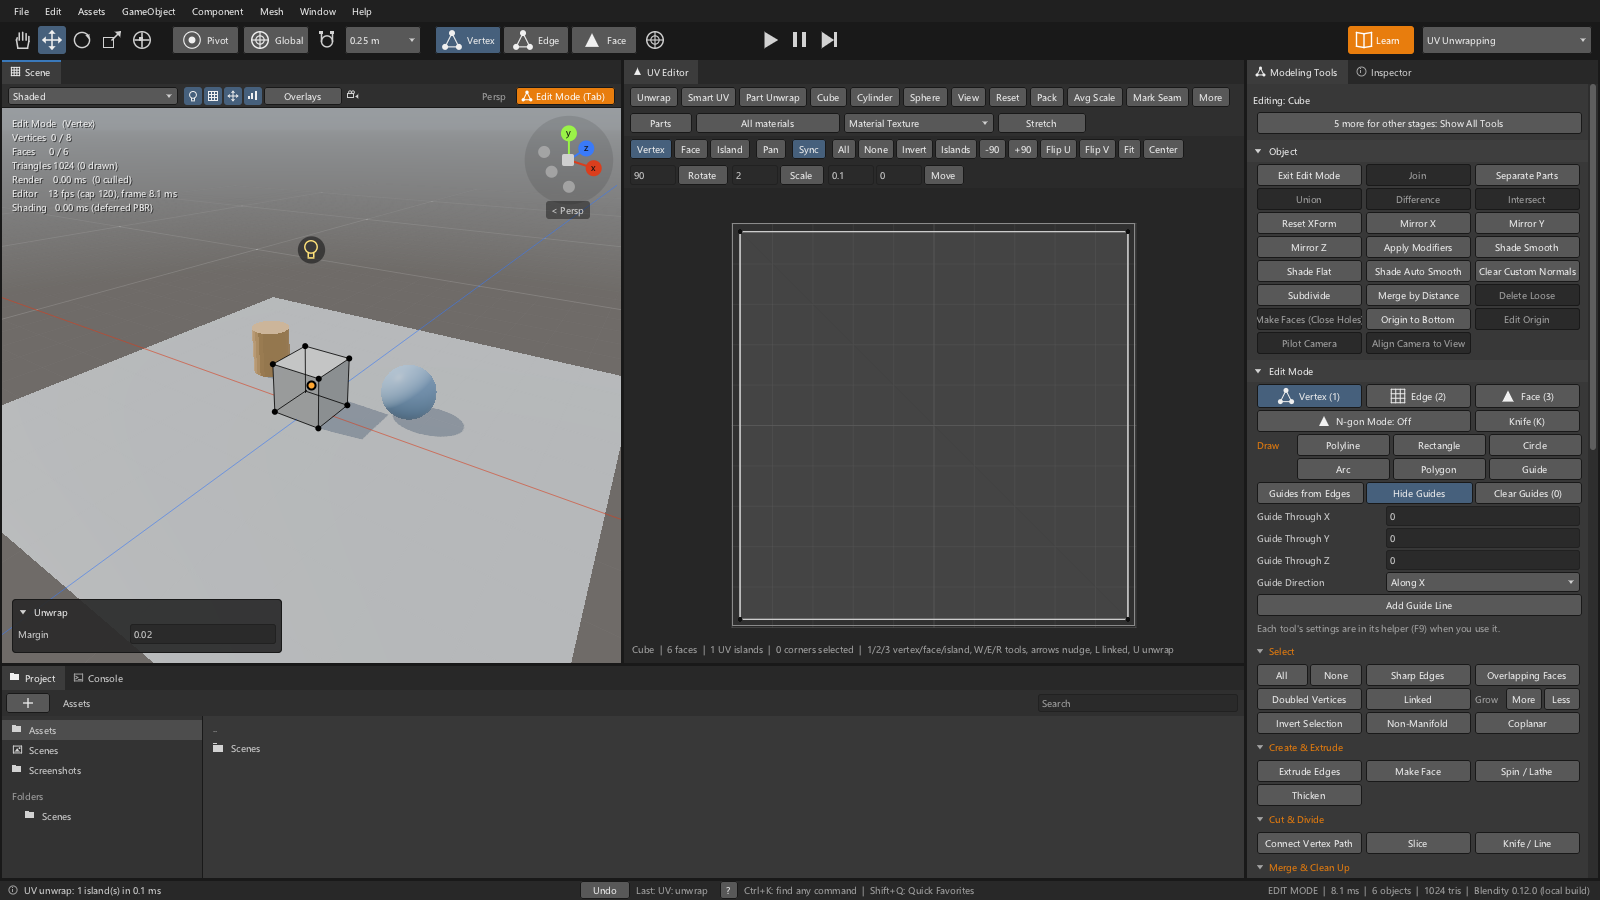
\includegraphics[width=\textwidth, alt={The UV Unwrapping layout: the Scene view with a cube in Edit Mode on the left, the UV Editor with its toolbar and the unwrapped cube's islands in the middle, the Modeling Tools window on the right.}]{layout-uv.png}
  \caption{The UV Unwrapping layout: Edit Mode on the cube, the UV Editor's toolbar (Unwrap, Smart UV, Part Unwrap, the
  projections, Pack, Mark Seam; vertex / face / island selection; the transforms) and the Modeling Tools beside it.}
\end{figure}

\begin{example}{a crate with a clean texture layout}
\begin{enumerate}
  \item Create a Cube; Edit Mode, select all, UV $>$ Cube Projection.
  \item Set the UV Editor's background to UV Grid (Blender's test image) to check that the squares stay square.
\end{enumerate}
\end{example}

\begin{fromnote}{Where it comes from}
Edit Mode's operators follow Blender's BMesh operators and editors
\cite{Blender2026, BlenderManual2026}; Push/Pull, inference and Follow are SketchUp's \cite{SketchUpHelp2026}; Follow,
Lathe and Slice are UModeler's \cite{UModelerDocs2026}; Shell, Draft, Radial Array and the construction planes are
Plasticity's \cite{PlasticityDocs2026}; the parametric shapes are ProBuilder's \cite{ProBuilderDocs2026}; the sculpt
brushes, masks and remeshers follow ZBrush and Sculptris \cite{ZBrushDocs2026, SculptrisDocs2026}; the theory is in
\cite{MarschnerShirley2021} (meshes, texture coordinates). Learn: \emph{Meshes: Vertices, Edges, Faces}, \emph{Edit
Mode: Modeling Like Blender}, \emph{Modifiers vs Components}, \emph{Advanced Modeling Tools}, \emph{Bevel, Bridge and
Push Through}, \emph{Sculpting}, \emph{UV Mapping}.
\end{fromnote}

\chapter{Materials, textures and painting}
\label{ch:surface}

\section{Materials}
Materials are Unity-style, evaluating Blender's \textbf{Principled BSDF}: base colour, metallic, roughness, specular,
normal and emission, with tiling and offset, surface types Opaque, Cutout, Transparent, Glass and Volume (Fog), the
folded \ui{Principled: Subsurface, Sheen, Coat} group (skin, cloth, lacquer; Anisotropic for brushed metal and hair), and
shading models PBR, Toon (five styles with painted shadow, highlight and rim control, shade maps, ramps, a face shadow
map, inner lines and hatching, an Outline component; the lilToon group for VRChat avatars \cite{lilToon2026}) and
Hand-painted. The \textbf{Materials} window shows every material as a sphere (a software-shaded preview, Blinn--Phong
\cite{Phong1975}): drag one onto an object (the face under
the mouse picks the slot) or onto a face in Edit Mode; \ui{Assign to Selection} does it for the selection. Material
assets (\code{Assets/Materials/<name>.mat}) are shared by every object that uses them, as in Unity; a Unity project's
\code{.mat} loads by its shader and is never written over. \textbf{Axis materials} pick top, side and bottom materials by
slope without UVs. \textbf{Fog}: Surface Type Volume (Fog) makes a closed mesh's inside fog with Blender's Principled
Volume fields; F12 with path tracing draws it truly.

\section{Procedural textures: Blender's nodes as layers}
Procedural textures (\code{Assets/Textures/<name>.ptex}) are a stack of layers, like Blender's modifier stack:
generators (Brick, Wood Floor, Tiles, Voronoi, Noise with Musgrave's types, Perlin Noise \cite{Perlin2002Improving},
Wave, Magic, White Noise, Gabor, Checker, Gradient, the anime background generators) and filters (Blur, Levels, Warp,
Edge Wear, Color Ramp, Map Range, Clamp, Math, RGB Curves, Separate Channel, Posterize, Cavity), each with a blend
mode (Blender's Mix modes, Photoshop's too). One texture gives albedo, normal, roughness and height maps and stays
sharp at any distance with Live Shading; its \ui{Physical Size} is the metres one tile covers. The \textbf{Textures}
window makes and edits them: \ui{New} lists presets by theme; every pattern has a folded \ui{Mapping} group (offset,
rotation, scale, Seamless); Add Layer has a search; \key{Alt}+click a layer's name to see the stack up to it;
right-click any field's name for \ui{Reset to Default}. Blendity has no node canvas: each Blender node is a layer, a
layer's option or a material field.

\begin{center}
\small
\begin{tabularx}{\textwidth}{lX}
\toprule
Blender node & In Blendity \\
\midrule
Texture Coordinate, Mapping & the material's Mapping (UV, Box / triplanar, Generated); a layer's Mapping group \\
Noise, Voronoi, Wave, Magic, White Noise, Gabor, Checker, Brick, Gradient & the layers of those names \\
Image Texture & the Image layer, or a material's Base Map \\
Sky Texture, Environment Texture & the Lighting window's Environment; the Sky Gradient layer \\
Mix Color & a layer's Blend \\
RGB Curves, Invert, Hue/Saturation/Value, Bright/Contrast & the RGB Curves, Invert, Hue / Saturation and Levels layers \\
Color Ramp, Map Range, Clamp, Math, Separate RGB / HSV & the layers of those names \\
Bump, Normal Map, Displacement & a texture's Height as its normal; the material's Normal Map; the Displace modifier \\
Principled BSDF, Glass, Transparent, Principled Volume & the material; Surface Type Glass, Transparent, Volume (Fog) \\
Toon BSDF, Shader to RGB & Shading Model Toon \\
Mix Shader, Light Path, Attribute, Geometry & not yet (an axis material mixes three materials by slope) \\
\bottomrule
\end{tabularx}
\end{center}

\begin{example}{a brick wall material}
\begin{enumerate}
  \item \menu{Window > Textures > New > Bricks}. Adjust the brick layer's fields; it already has an Edge Wear layer:
    raise it for worn corners.
  \item Select the wall and press \ui{Assign to Selection}: albedo, normal and roughness are set, with the tiling.
\end{enumerate}
\end{example}

\section{Painting the surface: the Substance Painter pipeline}
In order \cite{SubstancePainterDocs2026}:
\begin{enumerate}
  \item \menu{GameObject > Bake Mesh Maps\ldots} (or the Textures window's \ui{Bake All Maps}): the mesh's own normal,
    position, curvature, ambient occlusion and thickness baked into its UV layout on a worker, under
    \code{Assets/Textures/MeshMaps}.
  \item \menu{GameObject > New Surface}: a texture in the object's own UV space whose layers write colour, height,
    roughness, metallic and emission; \textbf{Fill} layers with a \textbf{mask stack} (a mesh map through levels,
    Noise, Blur, Levels, an Anchor to another layer's mask), the \textbf{smart masks} (edge wear, dirt, dust, metal edge
    wear, position gradient, thickness, Ground Dirt, Cavity, a Material ID Mask), \textbf{Group} layers. Editing a
    layer redoes only the layers above it inside the edited rectangle.
  \item \textbf{Paint Mode} (\menu{Modeling Tools > Paint}; \key{B} under the Adobe preset): a material brush paints
    colour, roughness, metallic, height and emission at once by projection; the far side and anything behind are left
    alone; the pen's eraser end erases; Mirror X / Y / Z; \ui{Bucket Fill} fills the group, island, material or object
    you click, or a gradient; \ui{Stencil} holds an image over the view; a stroke is one light undo step. \code{paint 2d
    on} paints on the Textures window's canvas instead.
  \item \textbf{Smart materials}: the Textures window's shelf applies a built-in (Worn Steel, Painted Metal, Rubber,
    Wood, Plastic, Concrete, Gold) on top of the surface, where its generators read \emph{this} object's mesh maps;
    \ui{Save as Smart Material} keeps a group of your own.
  \item \textbf{Export Textures\ldots} (the Textures toolbar): the texture set packed as glTF, Unity, URP, HDRP, Unreal,
    Poiyomi or lilToon reads it, or separate maps.
\end{enumerate}

\textbf{The hand-painted look.} When the light should live in the texture: \code{paint bakelight} bakes the mesh maps'
occlusion and a key light into a Multiply layer to paint over; the Paint section's \ui{Tip} (Round, Flat turned to the
drag, Bristle), \ui{Mode} (Paint, Smudge, Blend), \ui{Wet} (the brush carries the colour it went over
\cite{Baxter2004Impasto}), \ui{Jitter} and grain make the brush behave like paint; the palette row keeps swatches and
shades; set the material's Shading Model to \ui{Hand-painted} so every renderer shows the texture as painted.

\section{Stylized environments and the anime look}
\menu{Modeling Tools > Strokes} paints geometry: a click on a surface adds a card, a drag with Ribbon a strip, into one
Stroke object whose cards shade by their own facing, by the surface's normal, or away from a \ui{Canopy} centre so a
bush of flat cards reads as one round volume; \code{strokeobj grass} drops blades onto the ground. \menu{Modeling Tools
> Scatter} places instances of a named object by density with a painted mask. The World's Sun Disc, Horizon Band and
Fog finish the look in every renderer alike. For the 2D look: \ui{Camera Flatten} squashes a character's depth toward
the camera as Guilty Gear Xrd does \cite{Motomura2015}; \ui{View Angle Shapes} brings shape keys in by the camera's
angle; \ui{Anime Face Normals} gives a head a proxy so toon shadows fall as drawn shapes; a Lattice can face the camera;
the Anime and Manga camera filters add line art, halftone and paper.

\section{Bake Textures}
\ui{Bake Textures} turns everything an object's materials do into plain images on new UVs, so other programs show what
Blendity renders; on export, \ui{Bake Textures} does it for the file.

\begin{fromnote}{Where it comes from}
The Principled BSDF and the texture nodes are Blender's \cite{Blender2026, BlenderManual2026}; the layer stack, mesh
maps, smart masks and smart materials are Substance Painter's \cite{SubstancePainterDocs2026}; the painterly brush
simplifies IMPaSTo \cite{Baxter2004Impasto}; the toon look follows Guilty Gear Xrd \cite{Motomura2015}, MToon
\cite{MToon2026} and lilToon \cite{lilToon2026}; the theory is in \cite{MarschnerShirley2021} (texture mapping,
procedural textures) and \cite{Gregory2018vol2} (materials, textures and shaders). Learn: \emph{Materials and
Textures}, \emph{Blender's Shader Nodes in the Textures Window}, \emph{Fog with a Volume Material}, \emph{Working
Faster with Textures and Materials}, \emph{Painting the Surface}, \emph{The Hand-painted Look}, \emph{Stylized
Environments}, \emph{Flatten to the Camera}, \emph{Shapes by the Camera's Angle}.
\end{fromnote}

\chapter{Lighting and rendering}
\label{ch:light}

\section{Lights, the world and the views}
Lights are Directional, Point, Spot and Area, with an optional colour temperature in kelvin \cite{Kang2002Design};
\ui{Aim at Point} turns a light to shine at the surface you click. The Scene and Game views rasterize (deferred PBR with
sun shadows and image-based lighting), so editing stays fast. The world is a gradient, Blender's Hosek--Wilkie
physical sky \cite{Hosek2012Analytic} driven by the first Directional Light, an HDRI or a colour, with a sun disc, a
horizon band and distance fog; the view transforms are Standard, Filmic, ACES, Unity's ACES (the curve Unity's
post-processing applies \cite{Hill2016ACES}) and, with OpenColorIO, AgX and Blender's others. The sky, fog and ambient
light are edited in one place, the \textbf{Lighting} window.

\section{F12 and the Render window}
\key{F12} renders the active camera with either engine: \textbf{rasterized} with supersampling, or \textbf{path traced}
(Cycles-like: soft shadows, bounced light, glass, fog, depth of field, with Embree and OpenImageDenoise when Blender's
libraries are present, else Blendity's own BVH and \`A-Trous denoiser). The \textbf{Render} window (\key{F11}) has
resolution presets, the device (CPU, GPU Compute on any Vulkan GPU, OptiX on NVIDIA, or GPU + CPU together: path tracing
picks the faster device by itself and never overruns a small GPU's memory), samples, path guiding, Film $>$
Transparent, and saves PNG, JPEG, HDR or EXR. \ui{Render Camera Sequence} renders every camera marked In Sequence;
\ui{Render Animation} (\key{Ctrl+F12}) renders every frame of the sequence or the selected clip as numbered PNGs and an
H.264 MP4 beside them (ProRes and a VRChat-ready preset too; the dependency-free build offers Blender's libraries or an
\code{ffmpeg} on the PATH); \ui{Live Preview} re-renders a quick preview as you edit; the image pans with a left drag.
MoonRay, DreamWorks' renderer \cite{MoonRay2026}, is an optional download run as a program of its own.

\begin{figure}[H]
  \centering
  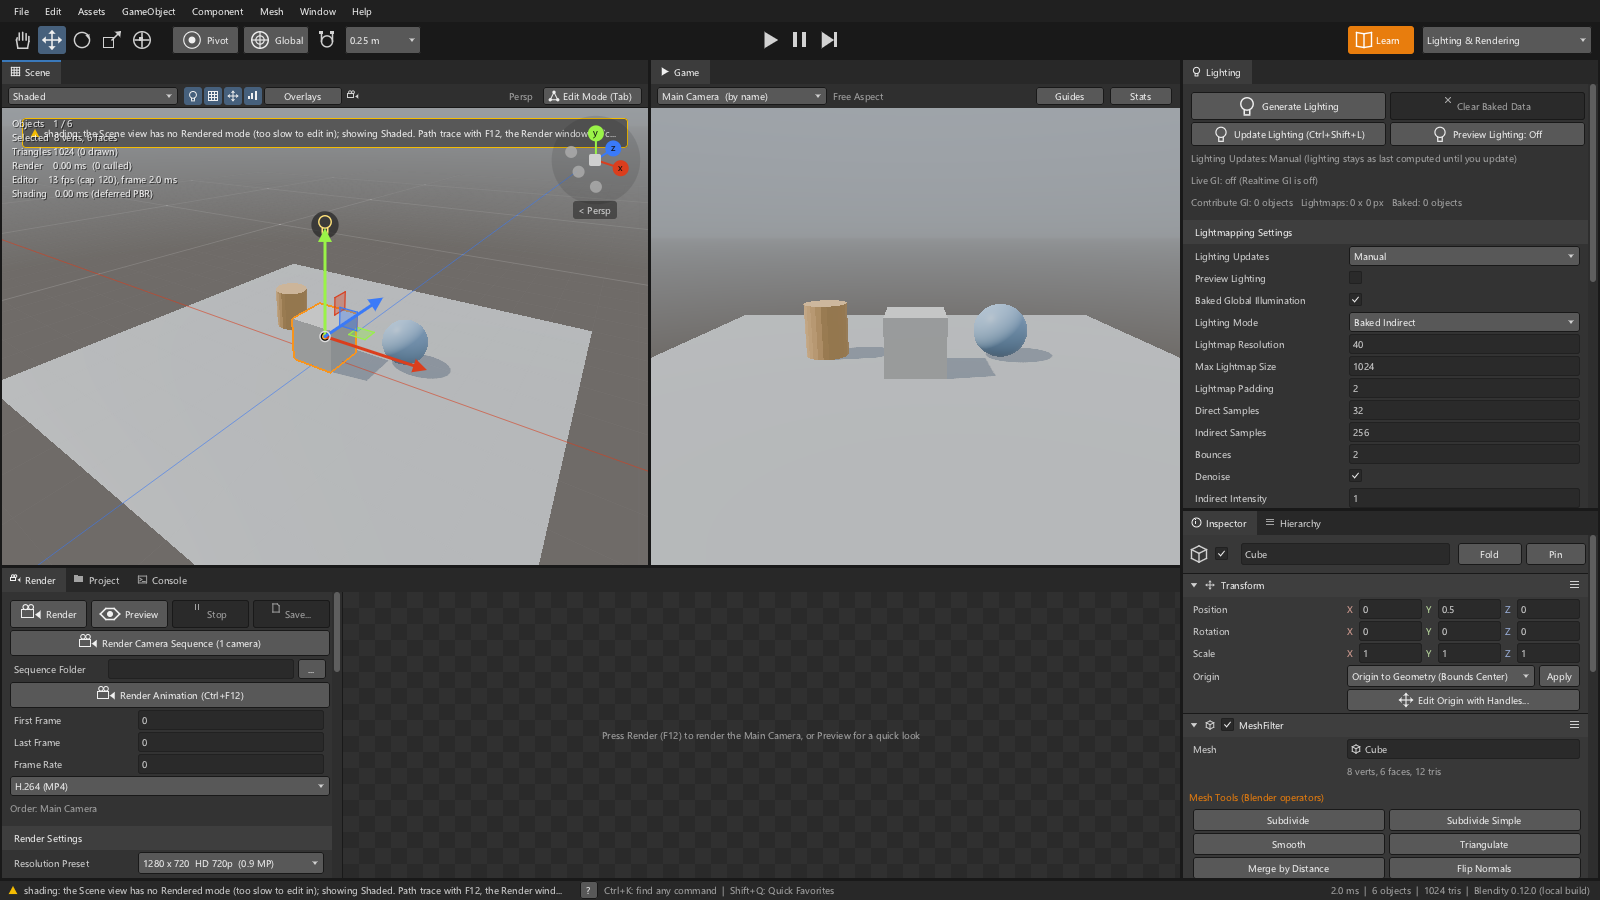
\includegraphics[width=\textwidth, alt={The Lighting and Rendering layout: the Scene view and the Game view side by side, the Lighting window with Generate Lighting and the lightmapping settings on the right, the Render window with its presets along the bottom.}]{layout-lighting.png}
  \caption{The Lighting \& Rendering layout: the Scene view, the Game view through the Main Camera, the Lighting
  window (Generate Lighting, the lightmapping settings) and the Render window with its presets.}
\end{figure}

\section{Baked, mixed and realtime light}
The short version for a scene that doesn't lag, as Unity does it \cite{UnityManual2026}:
\begin{enumerate}
  \item \textbf{Static objects:} select everything that never moves and tick \ui{MeshRenderer > Contribute GI}
    (\ui{Mark Static Meshes} does it for a world). Lightmap UVs are made for you.
  \item \textbf{Lights:} set each light's \ui{Mode}: \emph{Baked} (everything baked), \emph{Mixed} (bounces baked, direct
    light and shadows live: the usual choice for the sun) or \emph{Realtime}.
  \item \textbf{Bake:} \menu{Window > Lighting > Generate Lighting}. A baked lightmap costs about 1~ms on a 1080p frame.
  \item \textbf{Moving objects} take their bounced light from a \ui{Probe Volume} component (add one and bake again);
    metal and glass reflect a \ui{Reflection Probe}'s cubemap inside its box.
  \item \ui{Auto Generate} bakes again a second after you stop editing; the status bar says ``Lighting out of date''
    until it does. The bake is saved next to the scene.
\end{enumerate}
\ui{Lighting Updates: Manual} (the default) keeps bounced light as last computed while you drag things; \ui{Update
Lighting} (\key{Ctrl+Shift+L}) refreshes it; \ui{Preview Lighting} shows a rough bake half a second after you stop.
\textbf{Realtime GI} (voxel global illumination \cite{Thiedemann2011Voxel}) shows bounced light while you're still
arranging, with nothing to bake, and runs 4 to 8 times faster on a Vulkan GPU; set Render $>$ Device to GPU Compute
and Generate Lighting bakes on the GPU too.

\begin{center}
\small
\begin{tabularx}{\textwidth}{lXX}
\toprule
Setting & What it does & When to change it \\
\midrule
Lightmap Resolution & texels per metre (Unity's default is 40) & lower for big scenes, higher for sharp contact shadows \\
Indirect Samples, Bounces & rays per texel; how many times light bounces & raise if noisy; 3 or 4 for interiors \\
GI Resolution, Realtime Resolution & the live GI's share of the screen; realtime lightmaps' texels per metre & Half for a cleaner Scene view; higher for small rooms \\
Indirect Intensity & scales the baked bounce & artistic control \\
GI Device, Voxel Resolution & where realtime GI gathers; 64, 128 or 256 voxels across the scene & CPU only to compare; higher for small detail \\
Probe Min / Max Spacing & probe density near geometry / in open space & lower min spacing for small rooms \\
\bottomrule
\end{tabularx}
\end{center}

\section{Camera filters}
Camera filters are Unity's post-processing stack as components on a camera (\ui{Add Component > Camera Filters},
then \ui{Add Filter}): colour grading, bloom, vignette, chromatic aberration, lens distortion, film grain, CRT,
pixelate, edge outline, sharpen, halftone, hatching, line art, paper, a colour ramp, and whole looks: \textbf{Retro
Console} (PlayStation, N64, Saturn, DOS: wobbling vertices, affine textures, dithered colour \cite{psxspx}) and
\textbf{Anime / Manga}. They show in the Game view, the Camera Preview, F12 (traced renders too) and camera sequences;
the Scene view can look through them.

\begin{example}{a PS1-style render}
\begin{enumerate}
  \item Select the camera, \ui{Add Component > Camera Filters}, \ui{Add Filter > Retro Console}, Console: PlayStation.
  \item \key{F12}: the wobbling vertices, affine textures and dithered colour show in the path-traced render too.
\end{enumerate}
\end{example}

\section{Developing a render: the Editing tab}
\menu{Window > Editing} (or the Editing layout) develops a render or an image the way Lightroom does: a stack of
adjustments (Exposure, Contrast, Highlights / Shadows, white balance, a Tone Curve, HSL, Clarity, Dehaze, Sharpen,
Noise Reduction, Vignette, Crop), each limited by a mask if you like (a gradient, a tone or colour range, a brush),
applied in linear light and never written into the source: \ui{Save} keeps the stack beside the image, \ui{Export}
writes the result, \ui{Use as Camera Look} gives the camera the same look live, \ui{Apply to Texture} puts an edit on a
texture.

\section{A scene opened from Unity}
A Unity scene opened here looks as its Game view does: its fog mode, skybox, camera flags, post-processing (the ACES
tonemapper, exposure, grading, bloom, vignette), the lights' shadows and cookies, its reflection probes, and Unity's own
baked lightmaps and light probes (\ui{Lighting > Use Unity's Lightmaps}, read by your installed Unity in the
background). The match is measured station by station against Unity's renders (\code{docs/hci/compare-unity-vrchat-2026-11.md}).

\begin{fromnote}{Where it comes from}
The rasterizer follows EEVEE and the path tracer Cycles \cite{Blender2026}; the lighting modes, lightmaps, probe
volumes and post-processing follow Unity \cite{UnityManual2026}; the physical sky is Hosek and Wilkie's
\cite{Hosek2012Analytic}; realtime GI is Thiedemann et al.'s \cite{Thiedemann2011Voxel}; the microfacet model and
its sampling are Cook--Torrance, Walter et al.\ and Heitz \cite{Cook1982Reflectance, Walter2007Microfacet,
Heitz2018Sampling}; the denoiser is Dammertz et al.'s \cite{Dammertz2010Edge}; path guiding is Ruppert et al.'s
\cite{Ruppert2020Robust}; the bloom is Jimenez's \cite{Jimenez2014}; the theory is in \cite{MarschnerShirley2021}
(ray tracing, Monte Carlo, tone reproduction) and \cite{Gregory2018vol2} (lighting, post-processing). Learn: \emph{How
This Editor Renders}, \emph{Lights and Materials}, \emph{Render Engines}, \emph{Light, Sky and Tone Mapping},
\emph{Baked and Realtime Lighting}, \emph{Rendering on the GPU}, \emph{Editing: Develop a Render}.
\end{fromnote}

\chapter{Rigging, skinning and animation}
\label{ch:animate}

\section{Skeletons and skins}
Bones are GameObjects with a Bone component under a root with an Armature, as Unity imports a character. A mesh
follows them through its \ui{Armature (Skin)} modifier: each vertex moves with the bones its vertex groups are named
after. Everything for characters is in the \textbf{Rigging} window: Skeleton, Skin, Transfer Weights, Vertex Groups,
Weight Paint, Auto-Rig, IK, Spring Bones, Anime Face Normals. Select a bone and drag its blue tail handle to aim and
stretch it; \key{Ctrl+E} extrudes a new bone from the tip; IK targets are boxes and poles diamonds, coloured by side
(left blue, right red); \ui{FK Controls} puts circles on bones to turn them by \cite{BlenderManual2026}.

\textbf{Automatic weights by inpainting} (Epic's method \cite{Abdrashitov2023Robust}): \ui{Bind: Automatic Weights}
gives each vertex that is clearly nearest one bone, and that the bone can see, to that bone; the rest get the
smoothest weights that agree with them, so nothing bleeds across a gap. \ui{Bind: Envelope} is the quick distance-only
binding. \ui{Transfer Weights} dresses a character: drag the rigged body onto \ui{From}; close matches copy the body's
weights and everything else is inpainted. \textbf{Weight Paint} fixes weights by hand (Add, Subtract, Draw, Blur, a
falloff, Mirror X; \key{Ctrl} or the pen's eraser subtracts).

\textbf{IK.} \ui{Add IK to Bone} on a shin or a forearm makes a target and a pole; \menu{GameObject > Rig > Humanoid /
Quadruped} makes a whole skeleton with IK; \ui{Auto IK} finds the limbs of an imported Mixamo, Unity or Rigify
skeleton by name; an IK constraint's Weight 0 is FK, and \ui{Switch to FK / IK} keeps the pose. \textbf{Auto-Rig with
markers} (Mixamo's way \cite{Mixamo2026}): select the mesh, \ui{Auto-Rig > Humanoid} or \ui{Quadruped}, click the
markers the diagram asks for (chin, wrists, elbows, knees, groin; Symmetry mirrors), then \ui{Build Rig}: the skeleton,
IK on every limb and the inpainted weights.

\begin{example}{rig a character in five minutes}
\begin{enumerate}
  \item Import or model the character standing in a T- or A-pose, facing +Z (Unity's forward).
  \item Select it; \ui{Rigging > Auto-Rig > Humanoid}. Click the chin, the left wrist, the left elbow, the left knee
    and the groin.
  \item \ui{Build Rig}. Select a hand's IK target and move it: the arm follows, the mesh with it.
  \item Fix any weight with Weight Paint (select the bone to paint its group).
\end{enumerate}
\end{example}

\textbf{Spring Bones} make hair, ears, tails and cloth strips swing after the animation (Stiffness, Damping, Gravity,
Radius and Collide against the body's capsules, Bend, Root To Tip, Separate, a Wind component), found automatically by
name on imported characters (Mixamo, VRM, Japanese rigs); \ui{Bake} writes the swing into a clip. \textbf{Soft tissue}
on one bone trails the body's acceleration and keeps its volume.

\section{The Animation window}
\menu{Window > Animation} is Unity's Animation window \cite{UnityManual2026}, a dopesheet laid out as Unity's: a
Summary row of every key, an object row per animated object, the property rows under it with their axes, each row a key
button and a value field you can type into.
\begin{enumerate}
  \item Select the object (a character's root, a door) and press \ui{Create}: it gets an \ui{Animation} component and a
    clip, \code{Assets/Animations/<name>.anim}.
  \item Turn on \ui{Record} (\key{Ctrl+Shift+K}). Move the playhead along the ruler and pose things with the gizmo or the
    Inspector: every change becomes a key at the playhead; right-click any Inspector field $>$ \ui{Insert Keyframe}
    (or \key{I} over it) keys a light's intensity, a material slot's colour, a modifier's amount, a blend shape's weight.
  \item Press play in the window (or turn on \ui{Preview} and scrub); in Play (\key{Ctrl+P}) the Animation component
    plays the clip: Loop, Once, Ping Pong or Clamp Forever, at any speed.
\end{enumerate}
\textbf{Keys:} click, \key{Shift}+click or a box to select; drag sideways to retime; \key{Delete}; \key{Ctrl+C} /
\key{Ctrl+V} at the playhead; \key{K} keys every track; comma and full stop step through the keys; right-click for
\ui{Auto} (Unity's Clamped Auto), \ui{Linear} or \ui{Constant}; \ui{Add Property} is a tree of the objects with their
components. \textbf{Curves}: the window's \ui{Curves} view shows how each value travels between keys; drag a key's
tangent handles (\ui{Free Smooth}), or right-click for \ui{Broken} (a bounce), \ui{Flat} (an ease) or \ui{Clamped Auto}.
A clip names objects by their path below the animated root, so it plays on any character with the same bone names;
IK runs after the clip, so animating the IK targets is enough for arms and legs. Animation on 2s or 3s holds frames
for the anime look.

\begin{figure}[H]
  \centering
  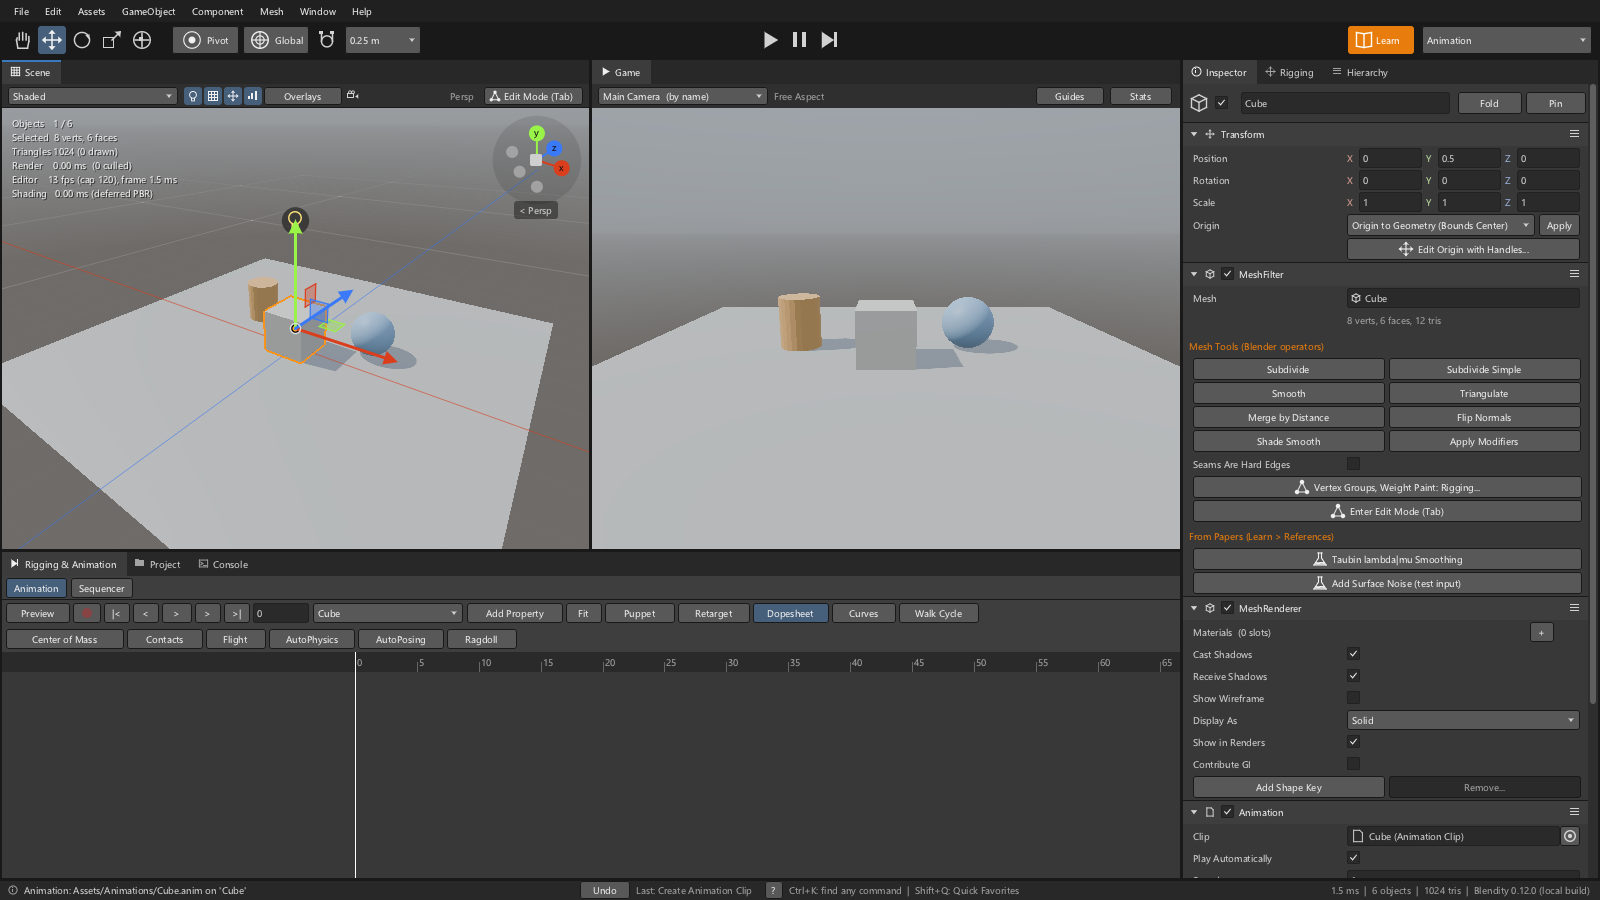
\includegraphics[width=\textwidth, alt={The Animation layout: the Scene view and the Game view above, the Animation window along the bottom with Preview, Record, the clip name, Add Property, Puppet, Retarget, Dopesheet and Curves, Walk Cycle and the physics tools, and the Rigging tab beside the Inspector.}]{layout-animation.png}
  \caption{The Animation layout: the Animation window along the bottom with Preview, Record, the clip, Add Property,
  Puppet, Retarget, Dopesheet / Curves, Walk Cycle and the physics tools; the Rigging tab beside the Inspector.}
\end{figure}

\begin{example}{a ball that bounces}
\begin{enumerate}
  \item Key the ball's Position y at 2 on frame 0, 0 on frame 15, 2 on frame 30.
  \item Curves view, click the Position.y track. Right-click the key on frame 15 $>$ \ui{Broken}.
  \item Drag its left handle steeply down and its right handle steeply up: the ball now hits the floor hard and leaves
    fast. Right-click the top keys $>$ \ui{Flat} for a hang at the top.
\end{enumerate}
\end{example}

\section{Puppet Posing and physics for animation}
Turn on \ui{AutoPosing} and the selected character's hands, feet, head and hips get controls in the Scene view: drag
one and the body follows, as motion capture would put a body there (a pose prior trained on the CMU database
\cite{Oreshkin2022Protores, CMUmocap2026}), the planted feet staying. Any humanoid rig works (Mixamo, the UE5 mannequin,
Character Creator, Daz, VRoid, Biped, Rigify; T or A pose). The \ui{Puppet} menu holds Reach, Motion Trails, Onion
Skin, the Zoetrope, Motion Check (sliding feet, pops and shaking, each with a Fix), the Smooth Brush and Lock in Place.
As in Cascadeur \cite{Cascadeur2026}: \ui{Center of Mass} weighs the body from its skin and follows it through a clip,
\ui{Contacts} are found from the motion and pinned, \ui{Flight} corrects a jump to a true parabola with its angular
momentum kept, \ui{AutoPhysics} makes the whole clip physically possible, take-offs and landings included, each shown
as a ghost before it is applied; \ui{Ragdoll} (Jolt) plays the clip with motors so hits and falls react. \ui{Walk Cycle}
makes walking and running cycles from the rig (feet never sliding, two legs or four), \ui{Footsteps} walks a character
along a curve on footprints you can move, \ui{Locomotion} walks and runs it live in Play. \ui{AI Inbetweening} (an
optional download) fills the motion between two keys in a style, shown as a ghost. Every assistant is a switch in
Preferences; hand animation never changes.

\section{Retargeting}
With a clip open on the rig it was made for, \ui{Retarget} lists the scene's other humanoid rigs; pick one and the clip
is remade for it by what each body part does (the 21 parts of the humanoid map found on any naming scheme), the hips'
moves scaled to its height and an A pose's arm drop reconciled with a T pose as Unity's Mecanim reads them
\cite{UnityHumanoidAvatars}; the new clip is saved beside the source's, set on the rig and opened. Fingers, the face
and IK are not carried.

\section{Sequencing clips}
\menu{Window > Sequencer} is a Premiere-style timeline for clips (instead of a state machine): press \ui{Create} and
drag \code{.anim} clips from the Project window onto its tracks; each bar is a clip and the object it plays on; drag
to move, its ends to trim; bars overlapping on one track crossfade; a higher track wins; \ui{Triggers} (a key, a clip,
blend seconds) jump to a clip in Play. The Sequencer also holds storyboard cards and camera cuts for animatics, WAV
sound mixed into Render Animation's video, footage, keyed opacity and transform, \ui{Add Edit} (\key{Alt+B}) and
\ui{Ripple Delete} (\key{Shift+Delete}).

\begin{fromnote}{Where it comes from}
Bones, skins and IK follow Blender's \cite{Blender2026, Welman1993Inverse}; the weights are Epic's inpainting
\cite{Abdrashitov2023Robust}; the marker auto-rig is Mixamo's workflow \cite{Mixamo2026}; the Animation window,
Record, the tangent modes, Humanoid retargeting and \code{.anim} clips are Unity's \cite{UnityManual2026,
UnityHumanoidAvatars}; the physics for animation follows Cascadeur's ideas \cite{Cascadeur2026}; the pose prior
follows ProtoRes \cite{Oreshkin2022Protores} on CMU data \cite{CMUmocap2026}; the spring chains follow Jakobsen and
the position-based solvers \cite{Jakobsen2001, Macklin2016}; the theory is in \cite{Gregory2018vol2} (animation,
physics). Learn: \emph{Modifiers vs Components} (vertex groups, weights, bones, IK, keyframes, curves, sequences),
\emph{Play Mode and the Game Loop}, \emph{Animating Any Property}.
\end{fromnote}

\chapter{Files, other programs and Live Link}
\label{ch:files}

\section{The project}
The Project window is \code{Assets}: nested folders, drag to move, \key{F2} to rename, \key{Delete} to the Recycle Bin
or Trash; references to a moved or renamed material, texture or clip keep working. Scenes are text files
(\code{.scene}); \key{Ctrl+S} saves, \ui{New} or \ui{Open} asks ``Save changes?'' first; the Console's \code{save},
\code{open} and \code{new} do the same.

\section{Import}
\menu{File > Import Model} (or drop files on the window): OBJ + MTL, FBX, glTF, STL, PLY and USD text, with their
materials and textures and, for rigged files, their skeletons, skins, bind poses, shape keys and animations
(\code{Assets/Animations/<model>/}); MikuMikuDance \code{.pmx} / \code{.pmd} characters rigged, toon-shaded and
dancing to \code{.vmd}; VRM avatars with their humanoid names, expressions, spring bones and MToon look; BVH motion
capture; Collada; \code{.blend} through your installed Blender. The \textbf{Import Preview} shows the model first with
its shading switchable (As Imported, PBR, or a toon style) and an Outline switch; Import writes it, Cancel nothing.
The texture finder reads the folders around the model and pairs each bare material with the texture set its name is
likeliest to own.

\section{Export}
\menu{File > Export}: every mesh format Blender 5.2 exports (OBJ, FBX binary or ASCII, glTF \code{.glb} or
\code{.gltf}, STL, PLY, USD) with Blender's options (Selected Only, Apply Modifiers, Scale, Up Axis, Triangulate, Keep
Transforms). glTF and FBX carry a rig, its skin, its clip and the shape keys (visemes, blinks and expressions reach
Unity, VRChat and Unreal); textures go with the file (procedural, painted and generated maps as PNGs, embedded in a
\code{.glb}); \ui{Lightmap UVs} adds a second UV set; \ui{Colliders} and \ui{LOD Levels} are named for Unity, Unreal or
Godot; \ui{Bake Textures} turns procedural materials into images; an export asked for while a remesh or a bind still
works on what it writes waits for it. Every format was checked both ways against Blender 5.2.

\section{Unity projects, VRChat, Godot, Blender, Unreal}
\textbf{Unity:} \menu{File > Import Unity Package\ldots} unpacks a \code{.unitypackage} into
\code{Assets/Imported/<package>/} with Unity's GUIDs kept; a prefab or a \code{.unity} scene comes in with its hierarchy,
meshes, materials (converted by shader: Standard, URP, lilToon, Poiyomi, MToon, UTS2), lights, cameras, colliders,
nested prefabs and overrides, and every other component as an Engine Component you can edit under Unity's names;
\menu{File > Open (Unity Scene)} opens a \code{.unity} as the scene with the look Unity gives it (chapter~\ref{ch:light});
Unity \code{.anim} clips import and export; \menu{File > Export Unity Package\ldots} writes the work back under the same
GUIDs. Nothing of Unity's is ever written over: an edit of a Unity clip or material saves to a Blendity copy beside it.

\textbf{VRChat:} the \textbf{Avatar} window (after the CATS plugin \cite{CATS2026}) has Fix Model, Create Visemes,
Model Options, Pose and Shape tools, Decimation, Bone Root and Bone Merging, Eye Tracking, the Texture Atlas, Merge
Armatures, Attach Mesh, Translate and Export for VRChat, with a checklist against VRChat's requirements
\cite{VRChatCreators2026}; the Profiler's \ui{Budget} ranks a scene or avatar against the PC and Quest performance
ranks; an avatar's VRChat components (the Avatar Descriptor, PhysBones, colliders, contacts, constraints) come in as
Blendity's and go back through the package or Live Link; a world's Scene Descriptor and Light Volumes too.

\textbf{Godot:} \code{.tscn} scenes come in with their nodes, primitives, materials, lights, cameras and collision
shapes and go back with the objects' transforms, scripts kept \cite{GodotDocs2026}. \textbf{Blender:} \code{.blend}
files come in through the installed Blender (\code{blender path} names it); the Blender bridge's \ui{Send to Blendity}
brings a scene over. \textbf{Unreal:} the bridge sends a level through its FBX exporter with each actor's place and
Blueprint class.

\section{Live Link}
Live Link sends the scene to Blender, Unity, Godot or Unreal \emph{as you work}: objects, transforms, meshes (a drag in
Edit Mode streams while it happens), materials, textures by their pixels, lights, cameras, a rig's poses and skins,
clips baked as the engine's own, colliders and LODs, the world and the render camera's look, VRChat's components where
the SDK is there. It starts with Blendity (Preferences $>$ Live Link) and writes where it listens, so a bridge connects
by itself. To put a bridge in: \menu{Window > Live Link > Install a Bridge} $>$ Blender (found and enabled for you), or
Unity / Godot / Unreal Project\ldots\ and pick the project's folder (in Unity: Package Manager $>$ Add package from
disk $>$ the bridge's \code{package.json}). The window lists who is connected. It is one way: edits on the other side
are not sent back. Work on a copy of a project you care about.

\begin{fromnote}{Where it comes from}
The formats follow Blender's importers and exporters \cite{Blender2026} and their specifications
\cite{Khronos2021Gltf, FBXBlender2026, USD2026}; Unity's files follow its manual \cite{UnityManual2026,
UnityPrefabsandtheYAMLsceneformat, UnityExportingapackage}; VRChat's limits and components follow its creator
documentation \cite{VRChatCreators2026}; the Avatar window follows CATS \cite{CATS2026}; Godot's format its
documentation \cite{GodotDocs2026}. Learn: \emph{Assets, Scenes and Files}, \emph{Coordinate Systems and Handedness}.
\end{fromnote}

\chapter{The Learn tab and the console}
\label{ch:learn}

\section{The Learn tab}
\key{F1} (or the orange \ui{Learn} button) opens the Learn tab; the Learning layout puts it beside the Scene view. Each
of its 45 lessons connects three layers: the Unity concept you can see on screen, the equivalent Blender concept with
the folder in Blender's source where it lives, and the theory behind it, cited from the reference books
\cite{MarschnerShirley2021, Gregory2018vol1, Gregory2018vol2} and the papers behind the features (the
\emph{References} lesson). Pick a lesson on the left; your progress is saved; \ui{Try it} buttons drive the editor for
you so you can watch the concept happen; click a question to reveal its answer; hover over almost any button or field
in the editor to see its Blender equivalent; the \ui{?} beside the status bar's hint opens the lesson for what you are
doing. Index C of this guide lists every lesson with its sources.

\begin{figure}[H]
  \centering
  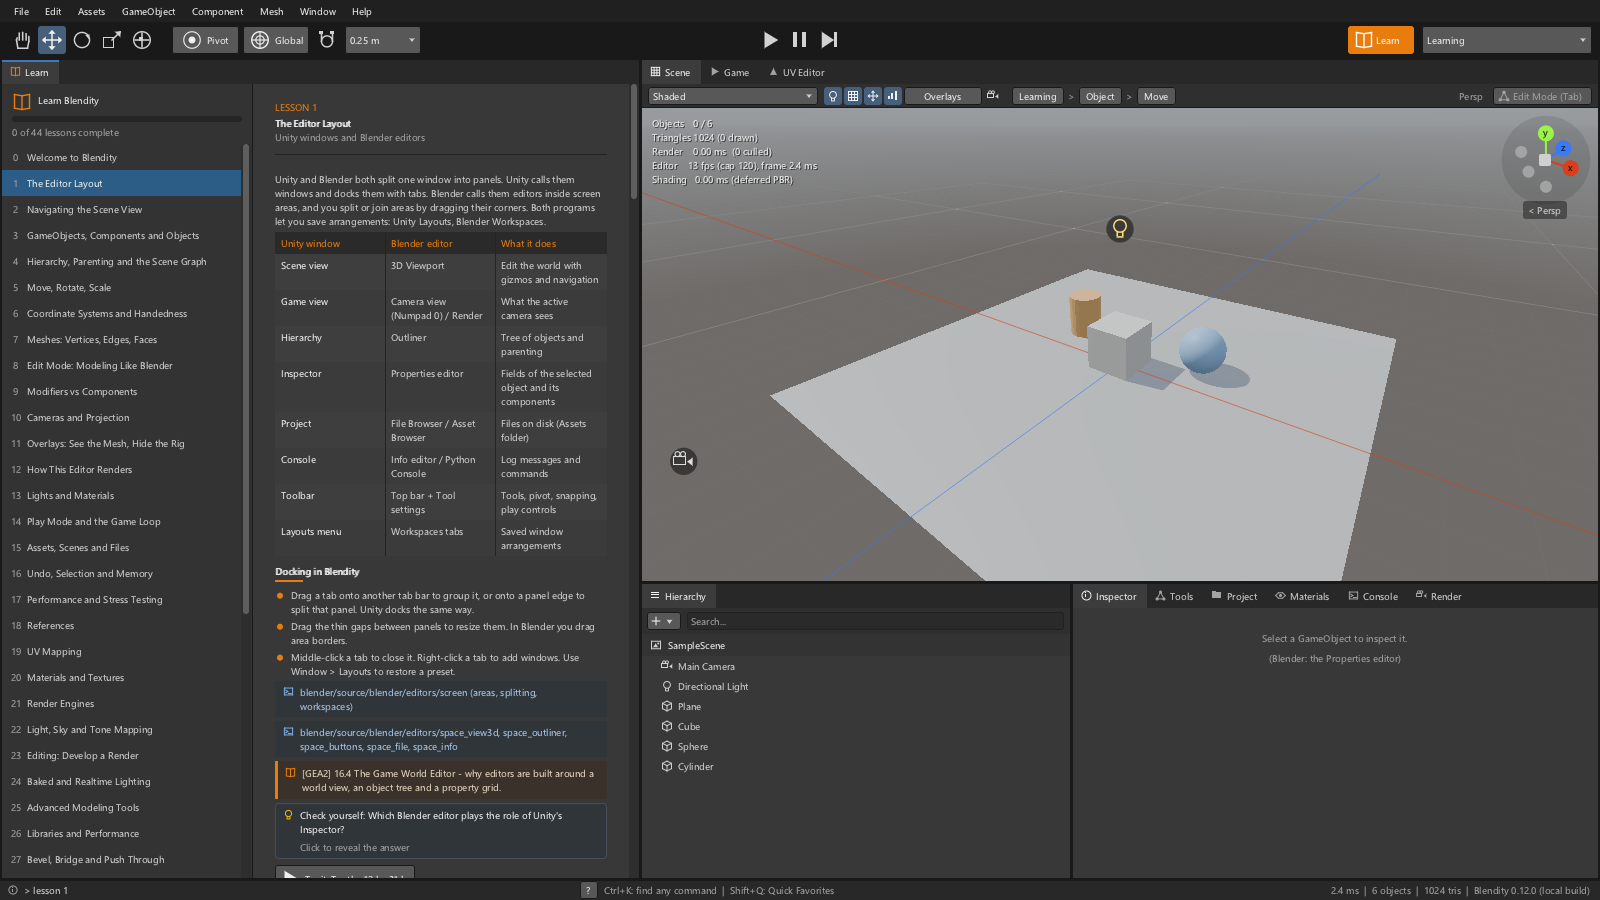
\includegraphics[width=\textwidth, alt={The Learning layout: the Learn tab's lesson list and a lesson with its table, references and Try-it buttons on the left, the Scene view the buttons drive on the right.}]{layout-learning.png}
  \caption{The Learning layout: the lesson list, a lesson with its table, references and Try-it buttons, and the Scene
  view the buttons drive.}
\end{figure}

The lessons, in order: Welcome to Blendity; The Editor Layout; Navigating the Scene View; GameObjects, Components and
Objects; Hierarchy, Parenting and the Scene Graph; Move, Rotate, Scale; Coordinate Systems and Handedness; Meshes:
Vertices, Edges, Faces; Edit Mode: Modeling Like Blender; Modifiers vs Components; Cameras and Projection; Overlays;
How This Editor Renders; Lights and Materials; Play Mode and the Game Loop; Assets, Scenes and Files; Undo, Selection
and Memory; Performance and Stress Testing; References; UV Mapping; Materials and Textures; Render Engines; Light, Sky
and Tone Mapping; Editing: Develop a Render; Baked and Realtime Lighting; Advanced Modeling Tools; Libraries and
Performance; Bevel, Bridge and Push Through; Rendering on the GPU; Points, Lines, N-gons and Booleans; Drawing in
Perspective; Customizing the Editor; Sculpting; Painting the Surface; The Hand-painted Look; Stylized Environments;
Drawing like SketchBook; Papers; Blender's Shader Nodes in the Textures Window; Fog with a Volume Material; Working
Faster with Textures and Materials; Flatten to the Camera; Shapes by the Camera's Angle; Animating Any Property; The Books and the References.

\section{The console}
Every tool can be driven from the Console's command line (type \code{help}; \key{Up} and \key{Down} recall what you
typed; a mistyped command is answered with the nearest known ones), which is also how scripts and the tests drive the
editor. None of it is needed any more: every verb an artist uses has a menu item, a button or a field. A few that are
handy by hand:

\begin{center}
\small
\begin{tabularx}{\textwidth}{lX}
\toprule
Command & Does \\
\midrule
\code{set Camera.FStop 1.4} & sets any field of the selected objects' components (enums by text) \\
\code{layout UV Unwrapping}, \code{alltools on} & layouts and Show All Tools \\
\code{skin bind}, \code{skin transfer Body Shirt} & automatic weights, weight transfer \\
\code{autorig humanoid}, \code{autorig build} & the marker auto-rig \\
\code{anim new}, \code{anim frame 30}, \code{anim record on}, \code{anim retarget <rig>} & the Animation window \\
\code{meshmaps 1024 16}, \code{surface new}, \code{paint on}, \code{smat apply Worn Steel} & the paint pipeline \\
\code{export textures unity Exports/Crate --assign} & the texture set packed for Unity, assigned to the material \\
\code{sketch on}, \code{sketchguide perspective 3}, \code{sketchcanvas ground}, \code{sketchbuild box} & the sketch pen, its guides and canvases, solids from the lines \\
\code{sculpt on}, \code{sculpt brush clay}, \code{sculpt dynamesh 128}, \code{sculpt remesh 2000} & Sculpt Mode and the remeshers \\
\code{render wait}, \code{saverender out.png}, \code{renderanim 1 120 24} & a render held till done, saved; an animation \\
\code{import <file>}, \code{export glb Exports/Hero.glb}, \code{export unitypackage <folder>} & files in and out \\
\code{livelink start}, \code{livelink status} & Live Link \\
\code{libs}, \code{jobs}, \code{budget pc}, \code{keymap table} & the build's libraries, the running jobs, the VRChat budget, every preset's keys \\
\code{update check}, \code{update history}, \code{update install <tag>} & the updater \\
\code{vr start}, \code{vr sketch on}, \code{vr paint on} & the VR View \\
\bottomrule
\end{tabularx}
\end{center}

\section{Headless runs and scripts}
\code{Blendity --headless-screenshot out.png --size 1600x900 --cmd "<command>" \ldots --frames N} runs the commands
with no window and writes a picture; \code{BLENDITY\_PROJECT} and \code{BLENDITY\_TRASH} point it at a scratch project,
never your \code{Assets}. The figures in this guide, the tests and the Unity comparison harness are made that way.

\section{Checking how it works for you}
\code{docs/hci/checklist.md} lists 118 tasks across the editor, each with its steps, what should happen and a target
time; its interactive page times each task with a stopwatch and keeps your results so the slow ones can be improved
first. How the editor's ease of use was measured (the keystroke-level model \cite{Card1980Keystroke}, the Fitts audit
\cite{Fitts1954Information}, the walkthroughs \cite{Polson1992Cognitive}, the heuristics \cite{Nielsen1994Enhancing}) is
in \code{docs/hci/README.md}.

\chapter{Pen, fingers, the Draw tab, papers, the board and VR}
\label{ch:pen}

\section{Fingers and a pen on a 2-in-1}
Tablet Mode (the tab menu, or Preferences $>$ Pen and touch: Auto follows the laptop's fold) makes the targets half as
big again (7~mm for a pen), and then fingers navigate while the pen works: one finger drags to orbit (a flick glides
on), taps to select, double-taps to frame; two fingers pinch to zoom, drag to pan, twist to turn; one finger scrolls a
list; the pen selects, moves, draws and paints, its side button held orbits (\key{Shift} pans, \key{Ctrl} zooms), its
side button clicked, or the pen or a finger held still half a second, opens \textbf{the Wheel}: one radial menu with
Undo, Delete, Extrude, the brushes, sizes and symmetry of whatever mode you are in; right-click any menu row $>$ \ui{Add
to the Wheel} puts a command on it. A finger's press waits a moment before it counts, so a pinch never starts a box
select; a palm resting on the screen while the pen is near is ignored. On Linux fingers and pens come through XInput 2;
on a Mac the trackpad's pinch and twist navigate and a tablet's pen has its pressure and tilt. The pen's pressure drives
the sculpt and paint brushes (a Pressure Curve in the brush settings), its tilt turns Flatten's and Scrape's plane and
widens a drawing brush, its eraser end erases and inverts.

\section{A pen display's dial and express keys}
Pen displays such as XPPen's send their express keys as keyboard shortcuts and their dial as a key pair or the wheel;
Blendity answers them where the pen draws: \key{Ctrl -} / \key{Ctrl =} zoom about the pen, \key{[} / \key{]} the brush
size, \key{4} / \key{6} turn the canvas and \key{5} sets it upright (Krita's keys \cite{Krita2026}), \key{B} brush,
\key{E} eraser, \key{Space} held pans, \key{Ctrl 0} fits; \ui{More > Wheel / Dial} chooses what the wheel does.

\section{The Draw tab}
\menu{Window > Draw} is the pad: the scene from the Scene or the Game camera, or blank Paper, the pen drawing in that
perspective while the keyboard moves the view (the arrows, \key{A} / \key{D}, \key{W} / \key{S} orbit and dolly the
camera while the pen is up), every stroke placed in the scene where it was drawn. It works like SketchBook Pro's canvas
\cite{SketchBookDocs2026}: one slim toolbar (Undo, Redo, Brush, the color with its opacity, Size, Ruler, Ellipse,
Curve, Symmetry, Perspective, Steady Stroke, Predictive Stroke, Layers, the zoom and More), the pad zoomed, panned,
turned and flipped with the wheel, a middle-drag or \key{Space}+drag and two fingers, \key{Tab} to hide the tools. The
brush palette holds Pencil, Pen, Inker, Felt Pen, Marker, Airbrush and two erasers, with the puck (drag sideways for
the size, up and down for the opacity; \key{B} held and dragged puts it at the pen) and Brush Properties on a
double-click. The \textbf{Layers} window composites the sketch's layers as Photoshop does \cite{PhotoshopHelp2026}:
opacity, the 27 blend modes, groups, locks, Clip to the layer below, a layer mask from a selection; \ui{More > Select}
has rectangle and lasso selections (\key{Alt+Backspace} fills, \key{Delete} cuts, \key{Ctrl+D} deselects) and \key{Ctrl+T}
Free Transform; \ui{More > Shapes} has Rectangle, Ellipse, Polygon, Star and Illustrator's Pen with fills, artboards
and SVG in and out. \ui{Place in 3D} puts each stroke in the scene at the depth under the pen; \ui{Build} and \ui{Lift}
make geometry from the construction lines (chapter~\ref{ch:plan}).

\begin{figure}[H]
  \centering
  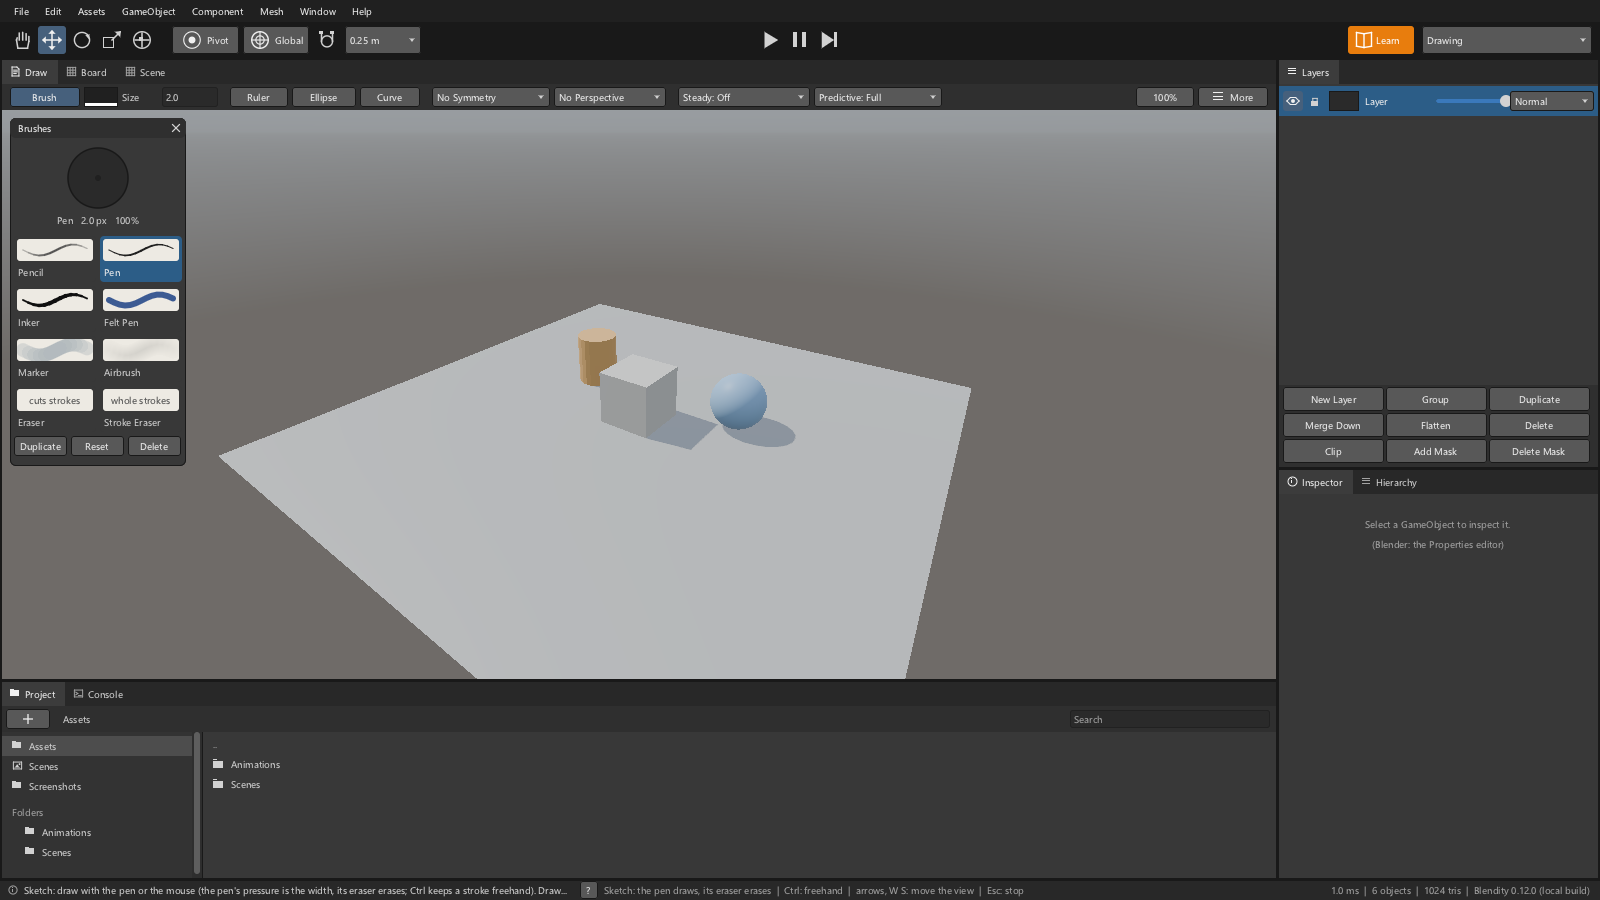
\includegraphics[width=\textwidth, alt={The Drawing layout: the Draw tab's pad with its slim toolbar at the top, the Layers window and the Project window.}]{layout-drawing.png}
  \caption{The Drawing layout: the Draw tab's pad with its toolbar, the Layers window and the Project window.}
\end{figure}

\section{Papers}
\ui{More > Source > Paper} draws on a paper: a page of its own in \code{Assets/Papers}, not in the scene. \ui{New Paper},
\ui{Open Paper}, \ui{Duplicate} and \ui{Delete} live under \ui{More > Paper}; a paper saves itself a second after each
change and on closing, and the one used last opens again. A paper can be pinned to the board, where double-clicking it
draws on it.

\section{The board}
\menu{Window > Board} is a PureRef-style reference board \cite{PureRef2026}: drop images from the system, drag them from
the Project window, \ui{Add Image\ldots} or \key{Ctrl+V} a screenshot; the wheel zooms about the pointer, a middle-drag
pans, \key{Home} fits everything, \key{F} frames the selection; drag to move, a corner to scale, the round handle to turn
(\key{Ctrl}: 15-degree steps); \key{Ctrl+]} / \key{Ctrl+[} to the front and back, \key{Ctrl+D} duplicates, \key{Delete}
removes; its own undo history; it saves itself to \code{Assets/Boards} and opens again next time; \menu{Boards >
Export\ldots} writes PNG, JPEG or PDF.

\section{VR View}
\menu{Edit > VR View} (\code{vr start}) shows the scene in an OpenXR headset (SteamVR, Quest Link, Windows Mixed
Reality \cite{OpenXR2026}) at life size, standing on the ground below where the Scene view looks. Squeeze a grip and
drag to move the world; both grips to scale or turn it; hold the right trigger to throw a teleport arc; the left stick
walks, the right snap-turns; \key{A} shows a tape measure. \code{vr sketch on}: the right trigger draws ribbons or tubes
in the air with pressure and a palette, into a Stroke object that renders and exports like any mesh. \code{vr paint
on}: paint the object with the desk's brush where the controller's ray meets it. It needs the build with Blender's
libraries, on Windows.

\begin{fromnote}{Learn}
\emph{The Editor Layout > Fingers and a pen on a 2-in-1}, \emph{Customizing the Editor}, \emph{Drawing like SketchBook},
\emph{Papers}, \emph{Drawing in Perspective}.
\end{fromnote}

\chapter{Performance, the minimum machine and troubleshooting}
\label{ch:trouble}

\section{The minimum machine and the quality tiers}
A thin laptop such as the HP Envy 13.3-inch 2-in-1 (an Intel i7 with 4 cores / 8 threads, 8~GB of RAM shared with
Iris Xe graphics, a 1920$\times$1080 touch screen at 150\,\%) runs Blendity on the \ui{Low} tier and says so on the
first run: editing frames at about 35--40 fps, orbiting at 60. A desktop with a 4-core CPU and a GTX 1050 Ti is faster.
The GPU is for path tracing, baking and realtime GI; a ray-tracing card (RTX, RX 6000+, Arc) is recommended for them.

\begin{center}
\begin{tabular}{lllll}
\toprule
Tier & Views drawn at & Shadow map & Frame cap & For \\
\midrule
Low & 67\,\% (scaled up) & 1024 & 60 fps & the minimum machine \\
Medium & 85\,\% & 2048 & 120 fps & a mid-range PC \\
High & 100\,\% & the scene's & 144 fps & a fast PC \\
\bottomrule
\end{tabular}
\end{center}

Renders (\key{F12}) always use the scene's own settings. \ui{CPU Threads} limits how many cores Blendity uses; the
\textbf{Profiler} window shows where a frame's time goes and its \ui{Budget} ranks the scene against VRChat's limits.
Tips for a scene that stays smooth: bake lighting, keep Lighting Updates on Manual, keep Subdivision Surface's Levels
at 1 while modelling, turn on the Low tier for heavy scenes, keep the Game view and the Camera Preview closed while
you don't need them (they keep their last picture during a drag anyway).

\section{When something refuses}
A refusal is a toast over the Scene view, and most carry a \ui{Fix}:
\begin{itemize}
  \item ``Edit Mode needs an active object with a MeshFilter'': select a mesh first.
  \item ``Paint needs a surface / UVs'': \ui{Fix} unwraps or makes the surface.
  \item ``\ldots\ can't run during Play'': \ui{Fix} stops Play.
  \item ``\ldots\ while a job runs on it'': the tray's \ui{Cancel}, or wait; an export waits by itself.
  \item ``Generate Lighting: no object contributes GI'': \ui{Mark Static Meshes}.
  \item A dim button: its tooltip says why (no selection, no libraries, the wrong mode).
  \item ``the Scene view has no Rendered mode'': path trace with \key{F12}; the Render window's \ui{Preview} is the quick look.
\end{itemize}

\section{Without Blender's libraries}
Preferences $>$ Libraries shows why a build runs without them (missing, damaged, turned off, offline) and offers
\ui{Download} or the switch. Without them: no Boolean or Decimate modifier, no EXR, no OpenColorIO views, slower path
tracing and the \`A-Trous denoiser, sphere physics in Play, and no MP4 of its own (Render Animation offers the
libraries or an \code{ffmpeg} on the PATH). Everything else works the same.

\section{The GPU}
A \ui{CPU} badge in the Scene view's bar says the views draw on the CPU although Auto wanted the graphics card; its
tooltip says why (no Vulkan, a material or world the card doesn't draw yet: volumes and the Principled extras go to the
CPU and say so). Render $>$ Device picks the path tracer's device; \code{gpu list} names the cards; a small GPU gets a
quarter of the RAM and is never overrun.

\section{Files and projects}
Your project is a folder with \code{Assets} inside; copy it whole. A scene names its materials, textures and clips by
project path and keeps values as a fallback, so a scene opened without its assets still shows. The Project window's
moves and deletes keep references working; deletes go to the system's trash. Never edit a Unity project you care
about in place: import a copy, or let Live Link write into a copy.

\section{Where to ask}
Open an issue on GitHub (\url{https://github.com/EmilianoManaloIV/blendity/issues}) with the Console's log (\ui{Copy}
in the Report dialog, or \code{BlendityProject/Screenshots} for a picture). If something in the documentation is out
of date, that is a bug too.

\begin{fromnote}{Learn}
\emph{Performance and Stress Testing > Quality tiers}, \emph{Rendering on the GPU > A small graphics card},
\emph{Libraries and Performance}.
\end{fromnote}

\chapter{Licensing and credit}
\label{ch:licensing}
Blendity follows Blender's design closely and is licensed to be compatible with it, with the libraries Blender bundles,
and with the way it is written: by an AI under a person's direction. This chapter states the licence terms once, the
reasoning behind them, and who is credited for what.

\section{The terms}
\begin{rulebox}{The licence, in four lines (\adr{0002}, \adr{0104})}
\begin{itemize}
  \item \textbf{The source} is GPL-2.0-or-later \cite{GPLv2}, the same as Blender's \cite{Blender2026}. Every source file
    carries \code{SPDX-License-Identifier: GPL-2.0-or-later} \cite{SPDX2024}; the full text is the root \code{LICENSE}.
  \item \textbf{The executables} are distributed under GPL-3.0-or-later \cite{GPLv3}, because they combine that source
    with Apache-2.0 code \cite{Apache2} (MikkTSpace, the Cycles sky evaluation, and when built with Blender's libraries
    Embree, OpenImageDenoise, oneTBB, Manifold, Open PGL and others), and Apache-2.0 combines with GPL version 3 but
    not with version 2 alone \cite{GPLFAQ2026}. This is Blender's own situation.
  \item \textbf{Your work is yours.} The GPL covers the program, not its output: scenes, meshes, textures, renders,
    animations and exported files belong to whoever made them.
  \item \textbf{Third-party notices} ship with every binary (\code{licenses/}), and any new copied code or library adds
    its row to \code{licenses/README.md} in the same change.
\end{itemize}
\end{rulebox}

\section{Why these terms are compatible with Blender's}
Blender is GPL-2.0-or-later. A program that borrows its design and ports pieces of its source must be under a licence
the GPL accepts, and ``GPL-2.0-or-later'' for the source keeps the two interchangeable in both directions: code could
move from Blender's tree into Blendity's and back without a relicensing. The ``or later'' clause is what lets the
binaries be GPL-3.0-or-later: Blender's own release binaries bundle the same Apache-2.0 libraries and are distributed
on the same basis.

Three kinds of third-party material are in or near the tree, each handled differently:
\begin{itemize}
  \item \textbf{Code copied unmodified from Blender's tree} into \code{extern/}: ufbx and fast\_float (MIT), MikkTSpace
    (Apache-2.0), the Hosek--Wilkie sky (BSD-3-Clause), QuadriFlow with LEMON and pcg32 (BSD-3-Clause, Boost, Apache-2.0),
    cuew (a modified Apache-2.0), \code{libc\_compat}. Their licence texts are in \code{licenses/} and
    \code{extern/README.md} says where each came from.
  \item \textbf{Code ported, not copied}: \code{src/render/sky.cpp} re-implements the sky radiance evaluation of Cycles'
    \code{intern/cycles/kernel/svm/sky.h} (Apache-2.0, 2011--2022 Blender Foundation) in Blendity's own functions. The
    file's header keeps that notice word for word, its SPDX line names both licences (\code{GPL-2.0-or-later AND
    Apache-2.0}), and the file as a whole is distributed under GPL-3.0-or-later through the ``or later'' clause
    (\adr{0002}, amended by \adr{0104}).
  \item \textbf{Code read, not copied}: lilToon's lighting formulas \cite{lilToon2026} are re-implemented from reading
    its shader (MIT; \adr{0100}); the Unity material converter reads Poiyomi's \cite{Poiyomi2026} and MToon's
    \cite{MToon2026} property names; the Avatar window follows the CATS plugin's tools \cite{CATS2026}; the physics for
    animation follows Cascadeur's ideas \cite{Cascadeur2026}. Nothing of their code is in the tree; they are credited
    in \code{CREDITS.md} and listed in \code{licenses/README.md} under ``read, not copied''.
\end{itemize}

\textbf{Optional downloads} are never part of a build: Blender's prebuilt libraries (fetched by the installer or by
Blendity itself, each under its own licence, all GPL-3-compatible), ONNX Runtime \cite{ONNXRuntime2026} and the
inbetweening network trained on the CMU motion capture database \cite{CMUmocap2026}, and MoonRay \cite{MoonRay2026}
run as a separate program (\adr{0041}). The Live Link bridges (\code{bridges/}) are Blendity's own code under the same
GPL-2.0-or-later and run inside Blender, Unity, Godot and Unreal as those programs' plug-in terms allow; they link no
code of Blendity's into them.

\section{Compatible with an AI-assisted project}
The code is written with Anthropic's Claude through Claude Code \cite{ClaudeCode2026} from task specifications and
decision records a person approves, and every change is reviewed by a person before it lands
(\code{docs/AI\_DISCLOSURE.md}). Three things make that compatible with the GPL and with reuse by others:
\begin{enumerate}
  \item \textbf{The outputs are the user's.} Under Anthropic's terms \cite{AnthropicTerms2026} the model's outputs belong
    to the user who directed them, and the project licenses them to the extent copyright subsists in them: the human
    selection, direction, review and editing (a purely machine-written passage may carry no copyright of its own, and
    the licence claims none it does not have). Copyright is held by Emiliano Manalo and contributors; the
    \code{Co-Authored-By} trailer names the model as attribution, not as a rights holder.
  \item \textbf{Nothing is claimed that isn't the project's.} Where a method comes from a paper, the paper is cited in
    the code's comments, in the Learn tab and in \code{research/FEATURES.md}; where code is copied, its licence rides
    along; where a program's design is followed, it is credited. A reader can tell, for every piece, what was borrowed
    and under what terms.
  \item \textbf{The AI is a tool at build time, not in the product.} The editor runs no model except the optional,
    local AI inbetweening download; there is no telemetry and no cloud, and the one request it makes on its own is the
    optional daily check of GitHub's releases. A user of the GPL program depends on no service.
\end{enumerate}

\section{Due credit}
Blendity stands on the work of others, and \code{CREDITS.md} names them: the Blender Foundation and the Blender authors,
whose design and source every subsystem follows \cite{Blender2026}; Unity Technologies, whose editor the windows,
shortcuts, Play mode, Animation window and asset formats follow \cite{UnityManual2026}; Epic Games (Unreal: the keymap
preset, the editor feel, FBX collision naming, Sequencer) \cite{UnrealDocs2026}; the Godot Engine contributors
\cite{GodotDocs2026}; Autodesk (Maya and 3ds Max presets) \cite{MayaDocs2026, MaxDocs2026}; Trimble (SketchUp's
Push/Pull, drawing and inference) \cite{SketchUpHelp2026}; Adobe (Photoshop's brush keys and blend modes, Substance
Painter's mesh maps and layer stacks, Mixamo's auto-rig) \cite{PhotoshopHelp2026, SubstancePainterDocs2026, Mixamo2026};
UModeler and Plasticity \cite{UModelerDocs2026, PlasticityDocs2026}; Maxon's ZBrush and Pixologic's Sculptris
\cite{ZBrushDocs2026, SculptrisDocs2026}; SketchBook \cite{SketchBookDocs2026}, PureRef \cite{PureRef2026} and Krita
\cite{Krita2026}; VRChat \cite{VRChatCreators2026}, lilToon \cite{lilToon2026}, Poiyomi \cite{Poiyomi2026}, the VRM
Consortium \cite{MToon2026}, VRoid \cite{VRoid2026}, the MMD community \cite{MMD2026} and the CATS plugin
\cite{CATS2026}; Nekki's Cascadeur \cite{Cascadeur2026}; DreamWorks' MoonRay \cite{MoonRay2026}; REDSIM's VRC Light
Volumes \cite{VRCLightVolumes2026}; Carnegie Mellon's motion capture database \cite{CMUmocap2026}; Marschner and
Shirley \cite{MarschnerShirley2021} and Gregory \cite{Gregory2018vol1, Gregory2018vol2}, whose books the Learn tab
teaches from; and the authors of every paper in the References chapter. Ideas are borrowed with their names attached;
code only with its licence.


\backmatter
% The reference list, by kind. Every entry is cited at least once (tools/make_books.py --check); the page numbers
% after an entry are where it is cited.
\chapter{References}
\label{ch:references}
Everything used in Blendity, by kind: the papers whose methods became features, the books the Learn tab teaches from,
the standards and licences, the libraries compiled in or linked, and the manuals of the programs Blendity follows.
Each entry ends with the pages that cite it. The list is generated from the sources that cite things
(\code{src/editor/lessons.cpp}, \code{research/FEATURES.md}, \code{licenses/README.md}) and a hand-written list
(\code{docs/book/refs\_extra.bib}); \code{tools/make\_books.py --check} fails when an entry is never cited or a citation
has no entry, so the list and the books cannot drift apart.

\printbibliography[keyword=papers, heading=subbibliography, title={Papers, theses and talks}]
\printbibliography[keyword=books, heading=subbibliography, title={Books}]
\printbibliography[keyword=standards, heading=subbibliography, title={Standards, specifications and licences}]
\printbibliography[keyword=software, heading=subbibliography, title={Software and libraries}]
\printbibliography[keyword=websites, heading=subbibliography, title={Manuals and websites}]

\chapter{Index C: the Learn lessons and their references}
\label{ch:indexC}
Each lesson of the Learn tab, the Blender source files it points to and the references it cites. Generated by
\code{tools/make\_books.py --bib} from \code{src/editor/lessons.cpp}; FoCG, GEA1 and GEA2 are the three reference books,
with the chapter each lesson sends you to.
% GENERATED by tools/make_books.py --bib. Do not edit: regenerate.

\begin{longtable}{>{\raggedright\arraybackslash}p{0.20\textwidth}>{\raggedright\arraybackslash}p{0.36\textwidth}>{\raggedright\arraybackslash}p{0.36\textwidth}}
\toprule \textbf{Learn lesson} & \textbf{Blender source it points to} & \textbf{References} \\ \midrule \endfirsthead
\toprule \textbf{Learn lesson} & \textbf{Blender source it points to} & \textbf{References} \\ \midrule \endhead
\bottomrule \endfoot
Welcome to Blendity & --- & \cite{MarschnerShirley2021,Gregory2018vol1,Gregory2018vol2} \\
The Editor Layout & blender/\allowbreak{}source/\allowbreak{}blender/\allowbreak{}editors/\allowbreak{}screen; blender/\allowbreak{}source/\allowbreak{}blender/\allowbreak{}editors/\allowbreak{}space\_view3d, space\_outliner, space\_buttons, space\_file, space\_info; blender/\allowbreak{}source/\allowbreak{}blender/\allowbreak{}editors/\allowbreak{}space\_view3d/\allowbreak{}view3d\_navigate.cc; blender/\allowbreak{}intern/\allowbreak{}ghost/\allowbreak{}intern/\allowbreak{}GHOST\_SystemWin32.cc & \cite{Gregory2018vol2,Blender2026} (GEA2 16.4 The Game World Editor - why editors are built around a world view, an object tree and a property grid.) \\
Navigating the Scene View & blender/\allowbreak{}source/\allowbreak{}blender/\allowbreak{}editors/\allowbreak{}space\_view3d/\allowbreak{}view3d\_navigate\_view\_rotate.cc; blender/\allowbreak{}source/\allowbreak{}blender/\allowbreak{}editors/\allowbreak{}space\_view3d/\allowbreak{}view3d\_navigate\_walk.cc & \cite{MarschnerShirley2021,Gregory2018vol1,Blender2026} (FoCG 8.1 Viewing Transformations, 8.3 Perspective Projection, 8.5 Field-of-View; GEA1 5.3 Matrices, 5.4 Quaternions - camera orientation is stored as a quaternion here and in Blender) \\
GameObjects, Components and Objects & blender/\allowbreak{}source/\allowbreak{}blender/\allowbreak{}makesdna/\allowbreak{}DNA\_object\_types.h; blender/\allowbreak{}source/\allowbreak{}blender/\allowbreak{}blenkernel/\allowbreak{}intern/\allowbreak{}object.cc & \cite{Gregory2018vol2,Blender2026} (GEA2 16.2 Implementing Dynamic Elements: Game Objects; GEA2 17.2 Runtime Object Model Architectures - object-centric vs property-centric designs) \\
Hierarchy, Parenting and the Scene Graph & blender/\allowbreak{}source/\allowbreak{}blender/\allowbreak{}editors/\allowbreak{}object/\allowbreak{}object\_relations.cc; blender/\allowbreak{}source/\allowbreak{}blender/\allowbreak{}editors/\allowbreak{}space\_outliner & \cite{MarschnerShirley2021,Gregory2018vol2,Blender2026} (FoCG 12.2 Scene Graphs; GEA2 17.6 Updating Game Objects in Real Time (dependencies between object updates)) \\
Move, Rotate, Scale & blender/\allowbreak{}source/\allowbreak{}blender/\allowbreak{}editors/\allowbreak{}transform; blender/\allowbreak{}source/\allowbreak{}blender/\allowbreak{}editors/\allowbreak{}gizmo\_library; blender/\allowbreak{}source/\allowbreak{}blender/\allowbreak{}editors/\allowbreak{}object/\allowbreak{}object\_transform.cc & \cite{MarschnerShirley2021,Gregory2018vol1,Blender2026} (FoCG 7.2 3D Linear Transformations, 7.3 Translation and Affine Transformations, 7.4 Inverses of Transformation Matrices; GEA1 5.3 Matrices, 5.4 Quaternions, 5.5 Comparison of Rotational Representations) \\
Coordinate Systems and Handedness & blender/\allowbreak{}source/\allowbreak{}blender/\allowbreak{}io/\allowbreak{}wavefront\_obj & \cite{MarschnerShirley2021,Gregory2018vol1,Blender2026} (FoCG 7.5 Coordinate Transformations; GEA1 5.2 Points and Vectors (left- vs right-handed coordinate systems)) \\
Meshes: Vertices, Edges, Faces & blender/\allowbreak{}source/\allowbreak{}blender/\allowbreak{}makesdna/\allowbreak{}DNA\_mesh\_types.h; blender/\allowbreak{}source/\allowbreak{}blender/\allowbreak{}blenkernel/\allowbreak{}intern/\allowbreak{}mesh\_normals.cc & \cite{MarschnerShirley2021,Blender2026} (FoCG 12.1 Triangle Meshes; FoCG 9.2 Operations Before and After Rasterization (interpolating attributes)) \\
Edit Mode: Modeling Like Blender & blender/\allowbreak{}source/\allowbreak{}blender/\allowbreak{}bmesh/\allowbreak{}operators/\allowbreak{}bmo\_extrude.cc; blender/\allowbreak{}source/\allowbreak{}blender/\allowbreak{}editors/\allowbreak{}mesh/\allowbreak{}editmesh\_extrude.cc; blender/\allowbreak{}source/\allowbreak{}blender/\allowbreak{}editors/\allowbreak{}transform/\allowbreak{}transform\_mode\_translate.cc & \cite{MarschnerShirley2021,Blender2026} (FoCG 12.1 Triangle Meshes (mesh connectivity)) \\
Modifiers vs Components & blender/\allowbreak{}source/\allowbreak{}blender/\allowbreak{}ikplugin/\allowbreak{}intern/\allowbreak{}iksolver\_plugin.cc; blender/\allowbreak{}source/\allowbreak{}blender/\allowbreak{}blenkernel/\allowbreak{}intern/\allowbreak{}subdiv\_mesh.cc; blender/\allowbreak{}source/\allowbreak{}blender/\allowbreak{}modifiers/\allowbreak{}intern/\allowbreak{}MOD\_smooth.cc & \cite{Welman1993Inverse,Abdrashitov2023Robust,Meyer2003Discrete,CATSCreateVisemes,VRChatAvatarDescriptorLipSync,CATSFixModel,UnityHumanoidAvatars,CATSModelOptionsandPosetools,CATSDecimationBoneRootandBoneMer,VRChatAvatarPerformanceRankingSyst,CATSEyeTrackingandMaterialCombin,VRChatAvatarDescriptorEyeLook,CATSCustomModelTranslateandExpor,UnityCollidercomponents,UnityLightingStaticGameObjects,UnrealFBXStaticMeshPipelinecollisi,UnityLODGroup,UnityImportingLODmeshes,UnrealSequencerCameraCutTrack,BlenderVideoSequencerSoundStrips,BlenderRenderOutputFFmpegVideo,UnityPrimitiveandplaceholderobjec,BlenderSculptingBrushStrokeUseTilta,UnityImportinglocalassetpackages,UnityPrefabsandtheYAMLsceneformat,lilToonPoiyomiMToonandUTS2Docs,VRChatPhysBones,UnityExportingapackage,GodotTSCNfileformat,GodotImporting3Dscenes,BlenderglTF20,UnrealExportinglevelstoFBX,Catmull1978Recursively,Blender2026} \\
Cameras and Projection & blender/\allowbreak{}intern/\allowbreak{}cycles/\allowbreak{}kernel/\allowbreak{}camera/\allowbreak{}camera.h; blender/\allowbreak{}intern/\allowbreak{}cycles/\allowbreak{}kernel/\allowbreak{}sample/\allowbreak{}mapping.h & \cite{MarschnerShirley2021,Gregory2018vol2,Blender2026} (FoCG 4.3 Computing Viewing Rays, 13.4 Choosing Random Points (on the aperture), 14.10 Monte Carlo Ray Tracing; FoCG 8.3 Perspective Projection, 8.4 Some Properties of the Perspective Transform, 8.5 Field-of-View; GEA2 11.2 Lights, Camera, Action!) \\
Overlays: See the Mesh, Hide the Rig & --- & \cite{UnityManual2026,BlenderManual2026} \\
How This Editor Renders & blender/\allowbreak{}source/\allowbreak{}blender/\allowbreak{}draw/\allowbreak{}intern/\allowbreak{}draw\_manager.cc; blender/\allowbreak{}source/\allowbreak{}blender/\allowbreak{}gpu/\allowbreak{}intern/\allowbreak{}gpu\_select.cc & \cite{MarschnerShirley2021,Gregory2018vol2,Gregory2018vol1,Blender2026} (FoCG 9.1 Rasterization, 9.2 Operations Before and After Rasterization, 9.4 Culling Primitives for Efficiency; GEA2 11.3 Foundations of 3D Rendering, 11.4 Programming the 3D Graphics Pipeline, 11.5 Pipeline Management; GEA1 4.3 Explicit Parallelism, 4.6 Thread Synchronization Primitives) \\
Lights and Materials & blender/\allowbreak{}intern/\allowbreak{}cycles/\allowbreak{}kernel/\allowbreak{}light/\allowbreak{}spot.h, blender/\allowbreak{}intern/\allowbreak{}cycles/\allowbreak{}kernel/\allowbreak{}light/\allowbreak{}area.h; blender/\allowbreak{}intern/\allowbreak{}cycles/\allowbreak{}kernel/\allowbreak{}svm/\allowbreak{}blackbody.h & \cite{MarschnerShirley2021,Gregory2018vol2,Blender2026} (FoCG ch. 5 Surface Shading; GEA2 12.3 The Rendering Equation, 12.4 The Shading Equation, 12.5 Lighting with Triangle Rasterization) \\
Play Mode and the Game Loop & --- & \cite{Gregory2018vol1,Gregory2018vol2,UnityManual2026,libJoltPhysics} (GEA1 8.2 The Game Loop, 8.5 Measuring and Dealing with Time; GEA2 14.3 The Collision Detection System, 14.4 Rigid Body Dynamics; GEA2 17.6 Updating Game Objects in Real Time) \\
Assets, Scenes and Files & blender/\allowbreak{}source/\allowbreak{}blender/\allowbreak{}blenloader/\allowbreak{}intern/\allowbreak{}writefile.cc; blender/\allowbreak{}source/\allowbreak{}blender/\allowbreak{}io/\allowbreak{}wavefront\_obj; blender/\allowbreak{}scripts/\allowbreak{}addons\_core/\allowbreak{}io\_scene\_gltf2/\allowbreak{}blender/\allowbreak{}imp/\allowbreak{}blender\_gltf.py; blender/\allowbreak{}source/\allowbreak{}blender/\allowbreak{}python/\allowbreak{}intern/\allowbreak{}bpy\_app\_timers.cc & \cite{Gregory2018vol1,Gregory2018vol2,Blender2026} (GEA1 7.1 File System, 7.2 The Resource Manager; GEA2 17.3 World Chunk Data Formats, 17.4 Loading and Streaming Game Worlds) \\
Undo, Selection and Memory & blender/\allowbreak{}source/\allowbreak{}blender/\allowbreak{}blenlib/\allowbreak{}BLI\_implicit\_sharing.hh; blender/\allowbreak{}source/\allowbreak{}blender/\allowbreak{}editors/\allowbreak{}undo & \cite{Gregory2018vol1,Blender2026} (GEA1 6.2 Memory Management, 6.3 Containers) \\
Performance and Stress Testing & --- & \cite{Gregory2018vol1,MarschnerShirley2021,Blender2026} (GEA1 2.3 Profiling Tools, 10.8 In-Game Profiling, 4.10 SIMD/Vector Processing; FoCG 12.3 Spatial Data Structures) \\
References & --- & \cite{Taubin1995Signal,Catmull1978Recursively,Levy2002Least,Mikkelsen2008Simulation,Newell1975Utilization,Thiedemann2011Voxel,Amanatides1987Fast,Cook1982Reflectance,Walter2007Microfacet,Heitz2018Sampling,Schlick1994Inexpensive,Karis2013Real,Heitz2018Combining,Shirley1997Low,Cranley1976Randomization,Wald2007Fast,Moller1997Fast,Duff2017Building,Ruppert2020Robust,Dammertz2010Edge,Hosek2012Analytic,Ramamoorthi2001Efficient,Kang2002Design,Perlin2002Improving,MarschnerShirley2021} (FoCG 11.5 Procedural 3D Textures) \\
UV Mapping & blender/\allowbreak{}source/\allowbreak{}blender/\allowbreak{}geometry/\allowbreak{}intern/\allowbreak{}uv\_parametrizer.cc; blender/\allowbreak{}source/\allowbreak{}blender/\allowbreak{}geometry/\allowbreak{}intern/\allowbreak{}uv\_pack.cc; blender/\allowbreak{}source/\allowbreak{}blender/\allowbreak{}editors/\allowbreak{}uvedit; blender/\allowbreak{}source/\allowbreak{}blender/\allowbreak{}geometry/\allowbreak{}intern/\allowbreak{}uv\_parametrizer.cc & \cite{Levy2002Least,MarschnerShirley2021,Wang2025Partuv,Sheffer2005Abf,Blender2026} (FoCG 11.2 Texture Coordinate Functions, 11.1 Looking Up Texture Values) \\
Materials and Textures & blender/\allowbreak{}source/\allowbreak{}blender/\allowbreak{}nodes/\allowbreak{}shader/\allowbreak{}nodes/\allowbreak{}node\_shader\_bsdf\_principled.cc; blender/\allowbreak{}intern/\allowbreak{}cycles/\allowbreak{}kernel/\allowbreak{}svm/\allowbreak{}checker.h, noise.h & \cite{MarschnerShirley2021,Gregory2018vol2,Blender2026} (FoCG 11.3 Antialiasing Texture Lookups, 11.4 Applications of Texture Mapping, 11.5 Procedural 3D Textures; FoCG 18.2 Color Spaces; GEA2 11.3 Foundations of 3D Rendering (textures, materials)) \\
Render Engines & blender/\allowbreak{}source/\allowbreak{}blender/\allowbreak{}draw/\allowbreak{}engines/\allowbreak{}eevee; blender/\allowbreak{}intern/\allowbreak{}cycles/\allowbreak{}kernel/\allowbreak{}integrator; blender/\allowbreak{}intern/\allowbreak{}cycles/\allowbreak{}bvh & \cite{Gregory2018vol2,MarschnerShirley2021,Blender2026} (GEA2 11.4 Programming the 3D Graphics Pipeline, 12.5 Lighting with Triangle Rasterization; FoCG 4 Ray Tracing, 12.3 Spatial Data Structures, 13.3 Monte Carlo Integration, 14.10 Monte Carlo Ray Tracing; GEA2 12.3 The Rendering Equation, 12.6 Lighting with Stochastic Ray Tracing) \\
Light, Sky and Tone Mapping & blender/\allowbreak{}intern/\allowbreak{}sky/\allowbreak{}source/\allowbreak{}sky\_hosek.cpp; blender/\allowbreak{}source/\allowbreak{}blender/\allowbreak{}imbuf/\allowbreak{}intern/\allowbreak{}colormanagement.cc & \cite{MarschnerShirley2021,Gregory2018vol2,Hosek2012Analytic,Blender2026} (FoCG 20 Tone Reproduction (20.2 Dynamic Range, 20.9 Sigmoids); FoCG 5.3 Ambient Illumination; GEA2 12.2 Radiometry and the Theory of Light Transport, 12.7 Post-Processing) \\
Editing: Develop a Render & --- & \cite{ASCCDL,ACES2026} \\
Baked and Realtime Lighting & blender/\allowbreak{}source/\allowbreak{}blender/\allowbreak{}draw/\allowbreak{}engines/\allowbreak{}eevee & \cite{Thiedemann2011Voxel,Gregory2018vol2,Blender2026} (GEA2 12.6 Lighting with Stochastic Ray Tracing) \\
Advanced Modeling Tools & blender/\allowbreak{}source/\allowbreak{}blender/\allowbreak{}bmesh/\allowbreak{}intern/\allowbreak{}bmesh\_walkers\_impl.cc; blender/\allowbreak{}source/\allowbreak{}blender/\allowbreak{}editors/\allowbreak{}mesh/\allowbreak{}editmesh\_loopcut.cc; blender/\allowbreak{}source/\allowbreak{}blender/\allowbreak{}modifiers/\allowbreak{}intern/\allowbreak{}MOD\_mirror.cc, MOD\_array.cc, MOD\_solidify\_extrude.cc & \cite{MarschnerShirley2021,Blender2026} (FoCG 12.1 Triangle Meshes (mesh connectivity), 12.2 Scene Graphs) \\
Libraries and Performance & blender/\allowbreak{}build\_files/\allowbreak{}build\_environment/\allowbreak{}cmake; blender/\allowbreak{}intern/\allowbreak{}cycles/\allowbreak{}bvh/\allowbreak{}embree.cpp, intern/\allowbreak{}cycles/\allowbreak{}integrator/\allowbreak{}denoiser\_oidn.cpp, intern/\allowbreak{}cycles/\allowbreak{}integrator/\allowbreak{}guiding.h; blender/\allowbreak{}source/\allowbreak{}blender/\allowbreak{}geometry/\allowbreak{}intern/\allowbreak{}mesh\_boolean\_manifold.cc; blender/\allowbreak{}intern/\allowbreak{}cycles/\allowbreak{}util/\allowbreak{}simd.h, blender/\allowbreak{}source/\allowbreak{}blender/\allowbreak{}blenlib/\allowbreak{}intern/\allowbreak{}math\_color.cc; blender/\allowbreak{}source/\allowbreak{}blender/\allowbreak{}blenlib/\allowbreak{}BLI\_task.hh & \cite{Gregory2018vol2,Gregory2018vol1,MarschnerShirley2021,Blender2026} (GEA2 14.2 Collision/Physics Middleware, 14.5 Integrating a Physics Engine into Your Game; GEA1 2.3 Profiling Tools; FoCG 22.3 Optimization Techniques; FoCG 9.4 Culling Primitives for Efficiency, 12.3 Spatial Data Structures; GEA1 4.10 SIMD/Vector Processing, 3.5 Memory Architectures, 3.3 Data, Code and Memory Layout; GEA1 4.3 Explicit Parallelism, 4.8 Some Rules of Thumb for Concurrency) \\
Bevel, Bridge and Push Through & blender/\allowbreak{}source/\allowbreak{}blender/\allowbreak{}bmesh/\allowbreak{}tools/\allowbreak{}bmesh\_bevel.cc, blender/\allowbreak{}source/\allowbreak{}blender/\allowbreak{}editors/\allowbreak{}mesh/\allowbreak{}editmesh\_bevel.cc; blender/\allowbreak{}source/\allowbreak{}blender/\allowbreak{}bmesh/\allowbreak{}operators/\allowbreak{}bmo\_bridge.cc; blender/\allowbreak{}source/\allowbreak{}blender/\allowbreak{}windowmanager/\allowbreak{}intern/\allowbreak{}wm\_operators.cc; blender/\allowbreak{}source/\allowbreak{}blender/\allowbreak{}editors/\allowbreak{}undo/\allowbreak{}ed\_undo.cc & \cite{MarschnerShirley2021,Gregory2018vol1,Blender2026} (FoCG 15.5 Cubics (the Hermite curve the tube follows), 12.1 Triangle Meshes; FoCG 21.5 Constructive Solid Geometry; GEA1 1.6 Tools and the Asset Pipeline) \\
Rendering on the GPU & blender/\allowbreak{}intern/\allowbreak{}cycles/\allowbreak{}device; blender/\allowbreak{}intern/\allowbreak{}cycles/\allowbreak{}kernel/\allowbreak{}integrator; blender/\allowbreak{}intern/\allowbreak{}cycles/\allowbreak{}session/\allowbreak{}session.cpp; blender/\allowbreak{}intern/\allowbreak{}cycles/\allowbreak{}integrator/\allowbreak{}path\_trace.cpp, blender/\allowbreak{}intern/\allowbreak{}cycles/\allowbreak{}integrator/\allowbreak{}work\_balancer.cpp; blender/\allowbreak{}intern/\allowbreak{}cycles/\allowbreak{}integrator/\allowbreak{}denoiser\_oidn.cpp, blender/\allowbreak{}intern/\allowbreak{}cycles/\allowbreak{}integrator/\allowbreak{}denoiser\_oidn\_gpu.cpp; blender/\allowbreak{}source/\allowbreak{}blender/\allowbreak{}gpu/\allowbreak{}opengl/\allowbreak{}gl\_debug.cc; blender/\allowbreak{}source/\allowbreak{}blender/\allowbreak{}editors/\allowbreak{}sculpt\_paint/\allowbreak{}mesh/\allowbreak{}sculpt.cc, blender/\allowbreak{}source/\allowbreak{}blender/\allowbreak{}draw/\allowbreak{}engines/\allowbreak{}eevee/\allowbreak{}eevee\_instance.cc & \cite{MarschnerShirley2021,Blender2026} (FoCG 12.3 Spatial Data Structures) \\
Points, Lines, N-gons and Booleans & blender/\allowbreak{}source/\allowbreak{}blender/\allowbreak{}bmesh/\allowbreak{}operators/\allowbreak{}bmo\_extrude.cc; blender/\allowbreak{}source/\allowbreak{}blender/\allowbreak{}editors/\allowbreak{}mesh/\allowbreak{}editmesh\_knife.cc; blender/\allowbreak{}source/\allowbreak{}blender/\allowbreak{}bmesh/\allowbreak{}operators/\allowbreak{}bmo\_dissolve.cc; blender/\allowbreak{}source/\allowbreak{}blender/\allowbreak{}geometry/\allowbreak{}intern/\allowbreak{}mesh\_boolean\_manifold.cc; blender/\allowbreak{}source/\allowbreak{}blender/\allowbreak{}editors/\allowbreak{}mesh/\allowbreak{}editmesh\_bisect.cc & \cite{Blender2026} \\
Drawing in Perspective & --- & \cite{Igarashi1997Interactive,Chen2013Sweep,Gryaditskaya2020Lifting,SketchBookDocs2026} \\
Customizing the Editor & source/\allowbreak{}blender/\allowbreak{}windowmanager & \cite{Gregory2018vol1,ZBrushDocs2026,BlenderManual2026,Blender2026} (GEA1 ch. 10 Tools for Debugging and Development - the tools pipeline; the editor is the first tool) \\
Sculpting & source/\allowbreak{}blender/\allowbreak{}editors/\allowbreak{}sculpt\_paint & \cite{MarschnerShirley2021,Gregory2018vol2,ZBrushDocs2026,SculptrisDocs2026,Jacobson2013Robust,Gibson1998Constrained,Huang2018Quadriflow,Blender2026} (FoCG ch. 12 Data Structures for Graphics - the half-edge and the triangle mesh the brushes walk; GEA2 ch. 10 The Rendering Engine - why a game wants the retopologized quads, not the sculpt) \\
Painting the Surface & source/\allowbreak{}blender/\allowbreak{}editors/\allowbreak{}sculpt\_paint/\allowbreak{}paint\_image\_proj.cc & \cite{MarschnerShirley2021,Gregory2018vol2,SubstancePainterDocs2026,Blender2026} (FoCG ch. 11 Texture Mapping - UV space, texel footprints and why a seam needs dilation; GEA2 ch. 10.6 Materials, textures and shaders in the rendering pipeline) \\
The Hand-painted Look & source/\allowbreak{}blender/\allowbreak{}editors/\allowbreak{}sculpt\_paint & \cite{MarschnerShirley2021,Gregory2018vol2,Baxter2004Impasto,Blender2026} (FoCG ch. 5 Linear Algebra and ch. 18 Color - value, hue and why the light can be premultiplied into the texture; GEA2 ch. 10.1 Foundations of Depth-Buffered Triangle Rasterization - the unlit path) \\
Stylized Environments & source/\allowbreak{}blender/\allowbreak{}editors/\allowbreak{}gpencil & \cite{MarschnerShirley2021,Gregory2018vol2,Blender2026} (FoCG ch. 15 Curves - the ribbon's strip along a path; ch. 11 Texture Mapping - the alpha-cut card; GEA2 ch. 10.4 Visual Effects and Overlays - particle and card systems, fog as a post effect) \\
Drawing like SketchBook & --- & \cite{SketchBookDocs2026,Krita2026,PhotoshopHelp2026} \\
Papers & --- & \cite{SketchBookDocs2026,PureRef2026} \\
Blender's Shader Nodes in the Textures Window & --- & \cite{Perlin2002Improving,BlenderManual2026} \\
Fog with a Volume Material & --- & \cite{BlenderManual2026} \\
Working Faster with Textures and Materials & --- & \cite{BlenderManual2026,SubstancePainterDocs2026} \\
Flatten to the Camera (the 2D Look) & --- & \cite{Motomura2015} \\
Shapes by the Camera's Angle & --- & \cite{Motomura2015} \\
Animating Any Property & --- & \cite{UnityManual2026,BlenderManual2026} \\
The Books and the References & --- & \cite{Gregory2018vol1} (GEA1 1.6 Tools and the Asset Pipeline - why an editor documents its pipeline and its sources) \\
\end{longtable}

\chapter*{Colophon}
\addcontentsline{toc}{chapter}{Colophon}
\textbf{Authorship and copyright.} Blendity is copyright Emiliano Manalo and contributors. Its source code, tests,
documentation and these two books were written with Anthropic's Claude through Claude Code \cite{ClaudeCode2026}, under
a human's direction and review: the user decides what Blendity is for, approves each task's specification and decision
record before code is written, reviews every pull request and merges it. The model's outputs belong to the user who
directed them under Anthropic's terms \cite{AnthropicTerms2026}, and are licensed to the extent copyright subsists in
them (the human selection, direction, review and editing); the \code{Co-Authored-By} trailer on every commit is
attribution, not a licence grant. No third-party code is claimed as the project's own: what is copied is listed in
\code{licenses/README.md} with its licence, what is followed is credited in \code{CREDITS.md} and the References
chapter, and the whole story is in \code{docs/AI\_DISCLOSURE.md}.

\textbf{Licence.} The source is GPL-2.0-or-later \cite{GPLv2}, the same as Blender's \cite{Blender2026}; the
executables, which combine it with Apache-2.0 libraries \cite{Apache2}, are distributed under GPL-3.0-or-later
\cite{GPLv3}. The scenes, meshes, textures, renders and animations made with Blendity are their maker's: the GPL covers
the program, not its output.

\textbf{How the books are made.} The sources are LaTeX under \code{docs/book/}, typeset with LuaLaTeX in the DejaVu
faces (the editor's own) and biblatex with biber for the reference list. \code{tools/make\_books.py} generates the
reference list and the index tables from the project's own files, takes the figures headless from a scratch project,
builds both PDFs and checks that nothing has drifted. The release workflow builds them again on every tag and attaches
them to the release.

\textbf{Accessibility and readability.} The books follow the guidelines the editor itself is measured against
(\adr{0085}), applied to documents: Nielsen's tenth heuristic, help and documentation \cite{Nielsen1994Enhancing,
Nielsen1993} (easy to search: a table of contents, bookmarks, a list of figures, a reference list with back-references
and three indexes; focused on the user's task: the user guide is the work stage by stage with numbered steps and worked
examples, the architecture book the questions a maintainer asks; not too large: each chapter ends in a pointer to the
Learn lesson that goes deeper); Carroll's minimalist instruction \cite{Carroll1990} (start on a real task, keep the
reading short, support error recovery: a troubleshooting chapter and the ``when something refuses'' list); and WCAG 2.1
\cite{W3C2018Web} as PDF/UA applies it \cite{PDFUA2024}: every text colour, link and box title reads at 4.5:1 or more
(the ratios are in \code{blendity-common.sty}), links are told apart by form as well as colour (bracketed citation
numbers, ``chapter 3'', monospace URLs), every figure carries alt text and a caption that says what it shows, the
diagrams' meaning is in their captions and the text around them, the document's language and metadata are declared
and its headings are the PDF's bookmarks (structure tags for a screen reader are the one open item: LaTeX's tagging
project does not yet support the packages the books use, so the captions carry what the alt text would), the body
type is about 10 points of a face made for screens with 80 characters a line, and nothing is conveyed by colour
alone. Keys, menus and controls are
typeset consistently: \key{Ctrl+K} is a key, \menu{Window > Layouts} a menu path, \ui{Generate Lighting} a control's
label, \code{make\_books.py} a file or command.

\textbf{Version.} Blendity 0.13.0, November 2026, from the \code{main} branch of
\url{https://github.com/EmilianoManaloIV/blendity}.

\end{document}
